\documentclass{article}

% Language setting
% Replace `english' with e.g. `spanish' to change the document language
\usepackage[utf8]{inputenc}
\usepackage{polski}

% Set page size and margins
% Replace `letterpaper' with `a4paper' for UK/EU standard size
\usepackage[letterpaper,top=2cm,bottom=2cm,left=3cm,right=3cm,marginparwidth=1.75cm]{geometry}

\usepackage{float}

% Useful packages
\usepackage{amsmath}
\usepackage{graphicx}
\usepackage[colorlinks=true, allcolors=blue]{hyperref}
\usepackage{listings}

% SQL Code Style
\lstdefinelanguage{SQL}{
    keywords={SELECT, INSERT, UPDATE, DELETE, FROM, WHERE, JOIN, ON, CREATE, TABLE, VALUES, INTO},
    keywordstyle=\color{blue}\bfseries,
    identifierstyle=\color{black},
    stringstyle=\color{red},
    commentstyle=\color{gray},
    morecomment=[l][\color{gray}]{--},
    sensitive=true
}

\lstset{
    language=SQL,
    basicstyle=\ttfamily\small,
    breaklines=true,
    keywordstyle=\color{blue},
    stringstyle=\color{red},
    commentstyle=\color{gray},
    showstringspaces=false,
}

\title{Baza danych medium społecznościowego}
\author{Łukasz Fabia 272724 \\ Mikołaj Kubś 272662 \\ Martyna Łopianiak 272682 \\ Piotr Schubert 272659 \\ Projektowanie baz danych wt 18:55}


\begin{document}
\maketitle

\tableofcontents

\section{Etap 1: Faza konceptualna}

\subsection{Analiza świata rzeczywistego}

\subsubsection{Streszczenie - Zarys wymagań projektu}

Celem projektu jest stworzenie bazy danych do obsługi medium społecznościowego. Ma ona przechowywać informacje o użytkownikach, ich treściach, relacjach i aktywnościach. Baza powinna być zaprojektowana w sposób wydajny i skalowalny.

\subsubsection{Potrzeby informacyjne}
\begin{itemize}
    \item Rejestracja i logowanie użytkowników z różnymi poziomami dostępu.
    \item Publikowanie i interakcje z treściami użytkowników (posty, polubienia, komentarze).
    \item Zarządzanie relacjami społecznymi (znajomości).
    \item Przechowywanie wiadomości prywatnych i historii aktywności.
    \item Tworzenie konwersacji z innymi użytkownikami
    \item Reportowanie postów z nieodpowiednimi treśćmi
    \item Tworzenie i zarządzanie stronami organizacji, firm, fanpage itd.
    \item Tworzenie i zarządzanie wydarzeniami
\end{itemize}

\subsubsection{Czynności, wyszukiwania}

\begin{itemize}
    \item Wyszukiwanie użytkowników.
    \item Wyszukiwanie treści po hasztagach lub słowach kluczowych.
    \item Filtrowanie aktywności użytkownika, np. przeglądanie polubień i komentarzy.
    \item Wyszukiwanie relacji (np. znajomi użytkownika, osoby obserwujące daną osobę).
    \item Dodawanie innych użytkowników do znajomych i interakcja z treściami - dodawanie komentarzy i reakcji
    \item Tworzenie postów, wydarzeń, grup
    \item Konwersacja grupowa, pisanie wiadomości
\end{itemize}

\subsubsection{Cele projektu}

\begin{tabular}{@{} l p{12cm} @{}}
    \textbf{S (Specific)}:   & Zaprojektowanie bazy danych dla medium społecznościowego.                                                                                                                                                                       \\ \\
    \textbf{M (Measurable)}: & Baza musi być wydajna, tzn. musi być w stanie obsługiwać dużą ilość użytkowników, co najmniej 20 000.                                                                                                                           \\ \\
    \textbf{A (Achievable)}: & Projekt zostanie zrealizowany przy użyciu PostgreSQL. Do stworzenia struktury tabel wykorzystany zostanie mechanizm ORM (Object Relational Mapping). Na koniec baza zostanie wypełniona danymi, aby przetestować jej wydajność. \\ \\
    \textbf{R (Relevant)}:   & Przechowywanie profili użytkowników oraz interakcje między nimi są kluczowe dla funkcjonowania medium społecznościowego.                                                                                                        \\ \\
    \textbf{T (Time-bound)}: & Praca nad projektem powinna zająć 2 miesiące.
\end{tabular}

\subsubsection{Zakres projektu}

\begin{tabular}{@{} l p{10cm} @{}}
    \textbf{Multimedia}:    & W bazie przechowywane będą wyłącznie linki do plików na zewnętrznym serwerze. \\
    \textbf{Obsługa haseł}: & Wszystkie hasła w bazie będą hashowane.
\end{tabular}


\subsection{Wymagania funkcjonalne}

\begin{abstract}
    Użytkownikom przypisany jest jeden z tych poziomów dostępu: admin, user lub guest.
\end{abstract}

\textbf{Guest(Gość)}

\begin{itemize}
    \item Może przeglądać wybrane dane.
\end{itemize}

\textbf{Admin}

\begin{itemize}
    \item Może przeglądać, edytować, usuwać, dodawać i przeglądać wszystkie treści, zrządza bazą i nadaje uprawnienia
\end{itemize}

\textbf{User(Użytkownik)}

\begin{itemize}
    \item System umożliwia rejestrację oraz logowanie.
    \item Rejestracja wymaga imienia, nazwiska, daty urodzenia, hasła oraz maila.
    \item Logowanie wymaga maila i hasła.
\end{itemize}


\subsection{ERD}

\begin{figure}[H]
    \centering
    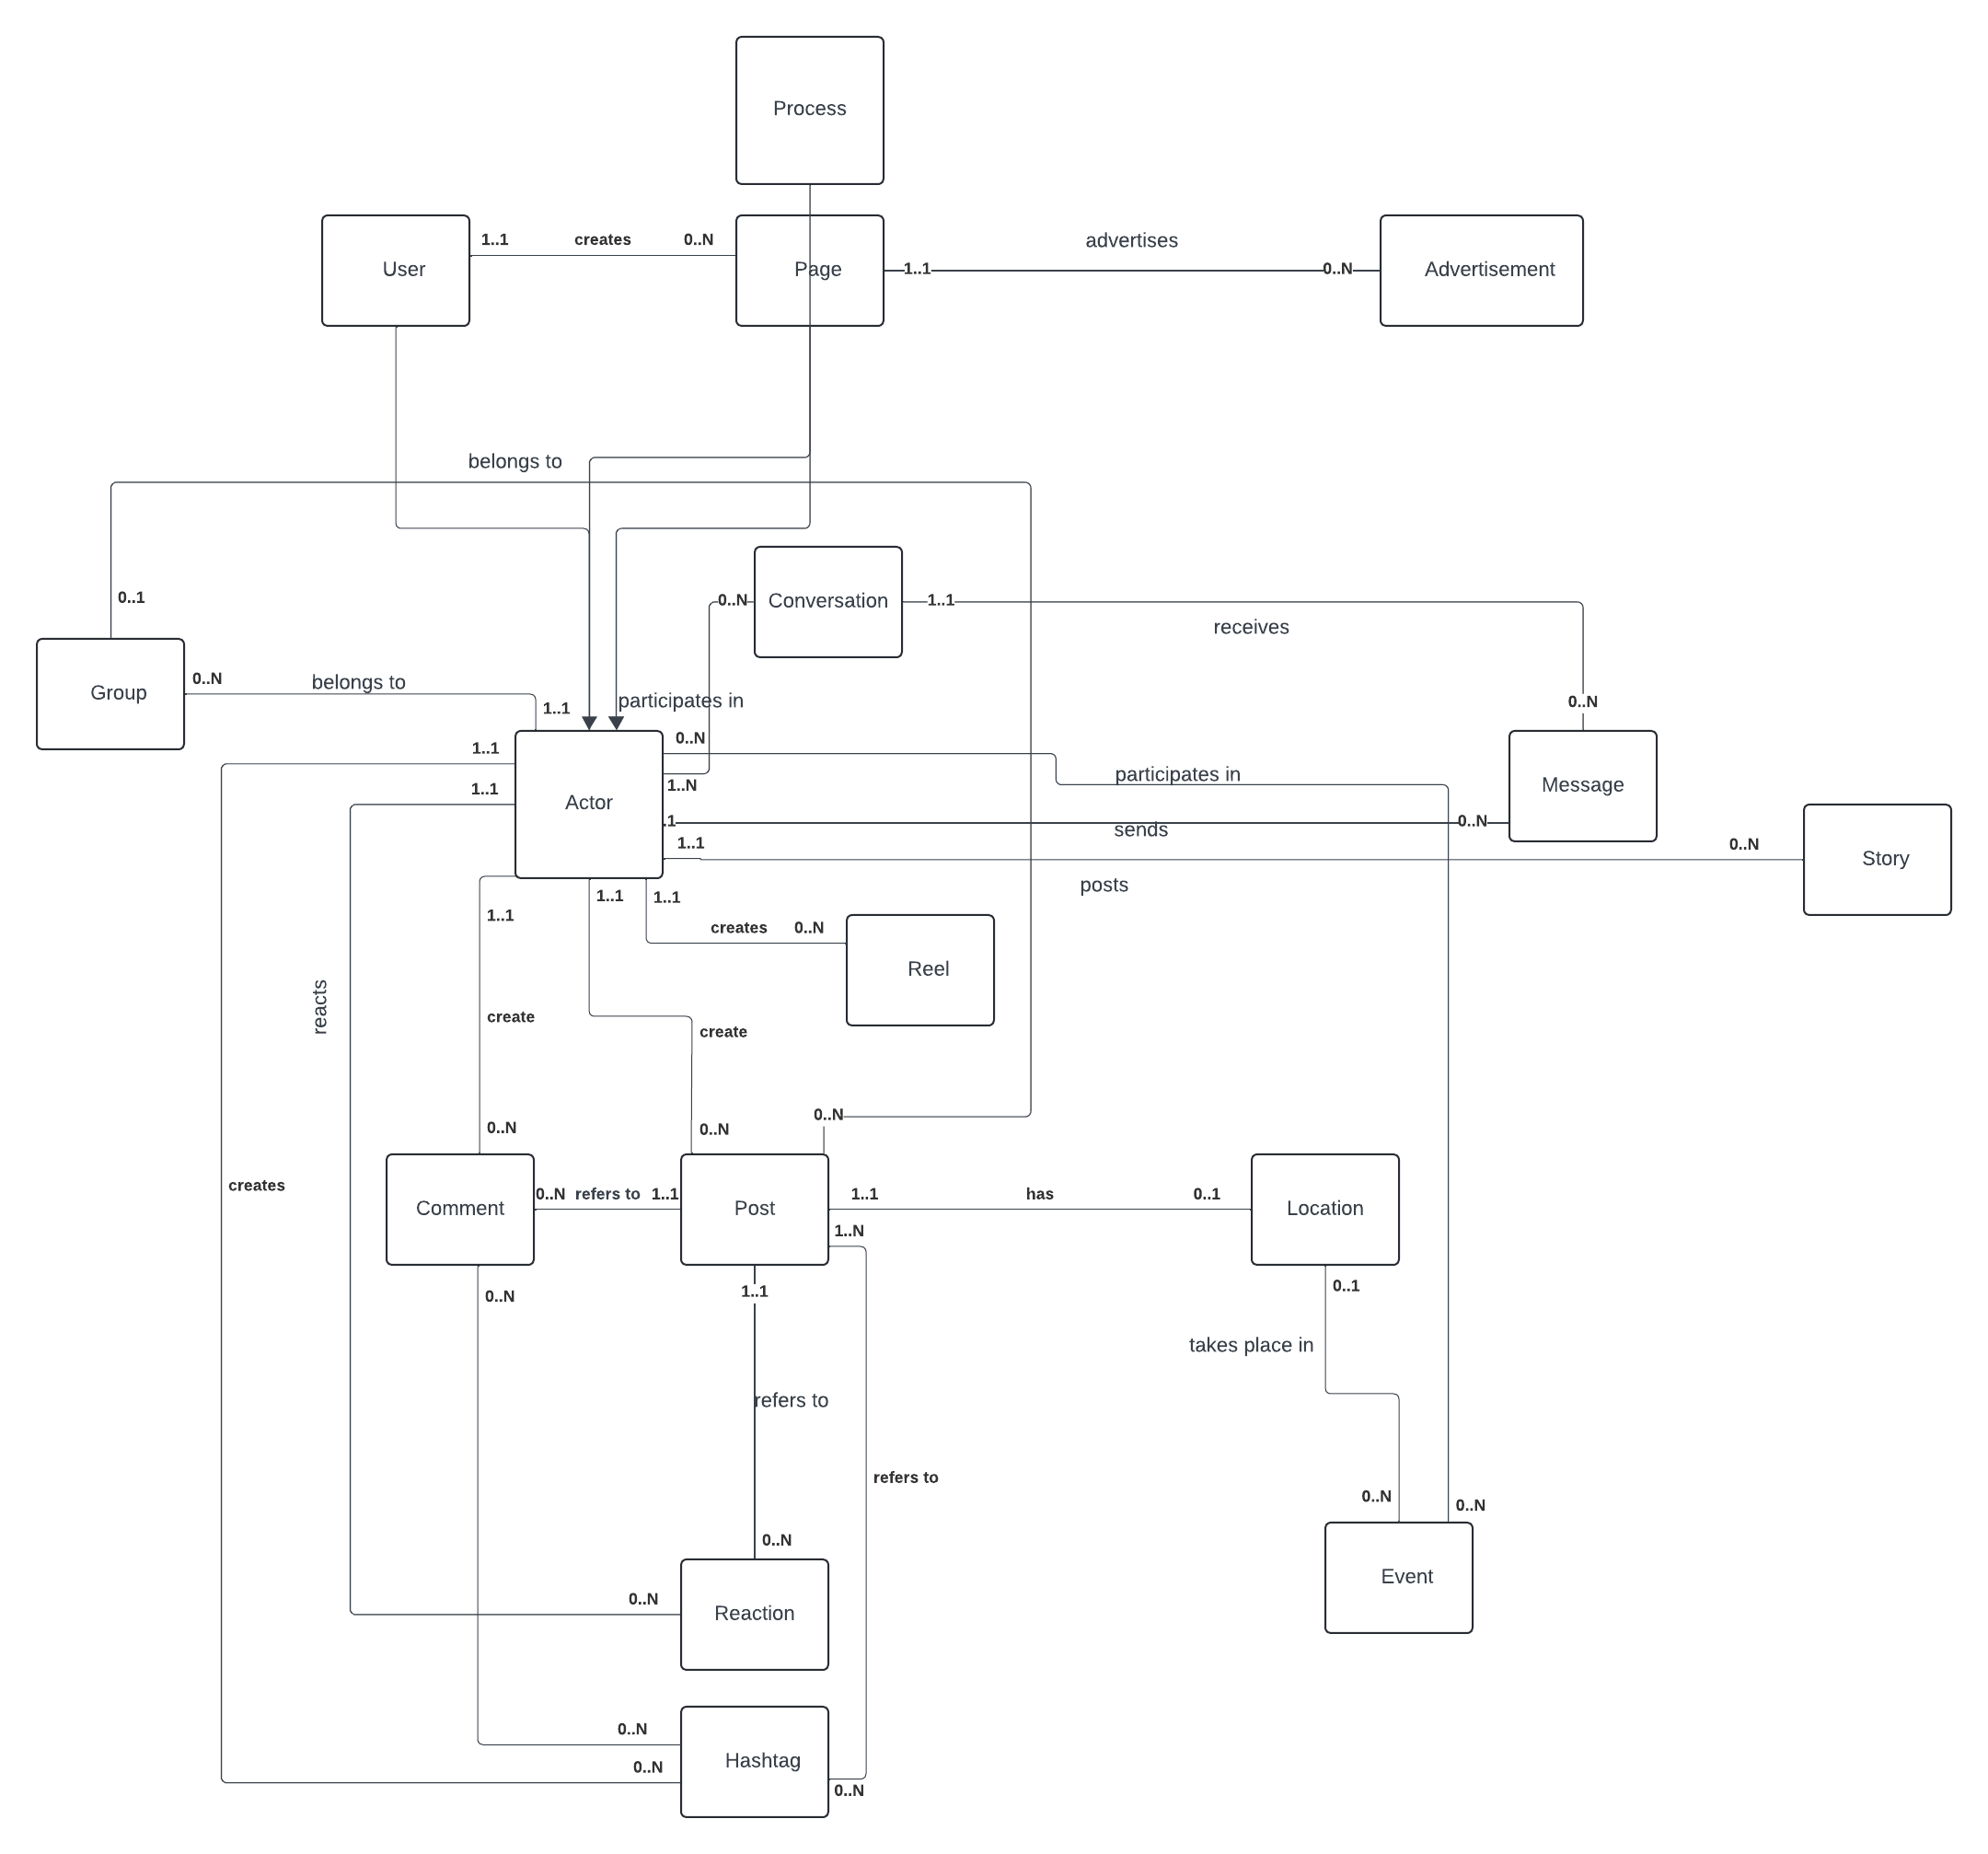
\includegraphics[width=\linewidth]{images/Blank diagram.png}
    \caption{Diagram obiektowo-relacyjny}
    \label{fig:erd}
\end{figure}

\section{Etap 2: Faza logiczna}

Do tabel zostały dodane atrybuty, tabele \textbf{Page} oraz \textbf{User} zostały uogólnione przez \textbf{Author}, który bierze udział w innych czynnościach. Baza została także sprowadzona do \textit{III postaci normalniej}, przez co wydzielono klika nowych tabel.

\begin{figure}[H]
    \centering
    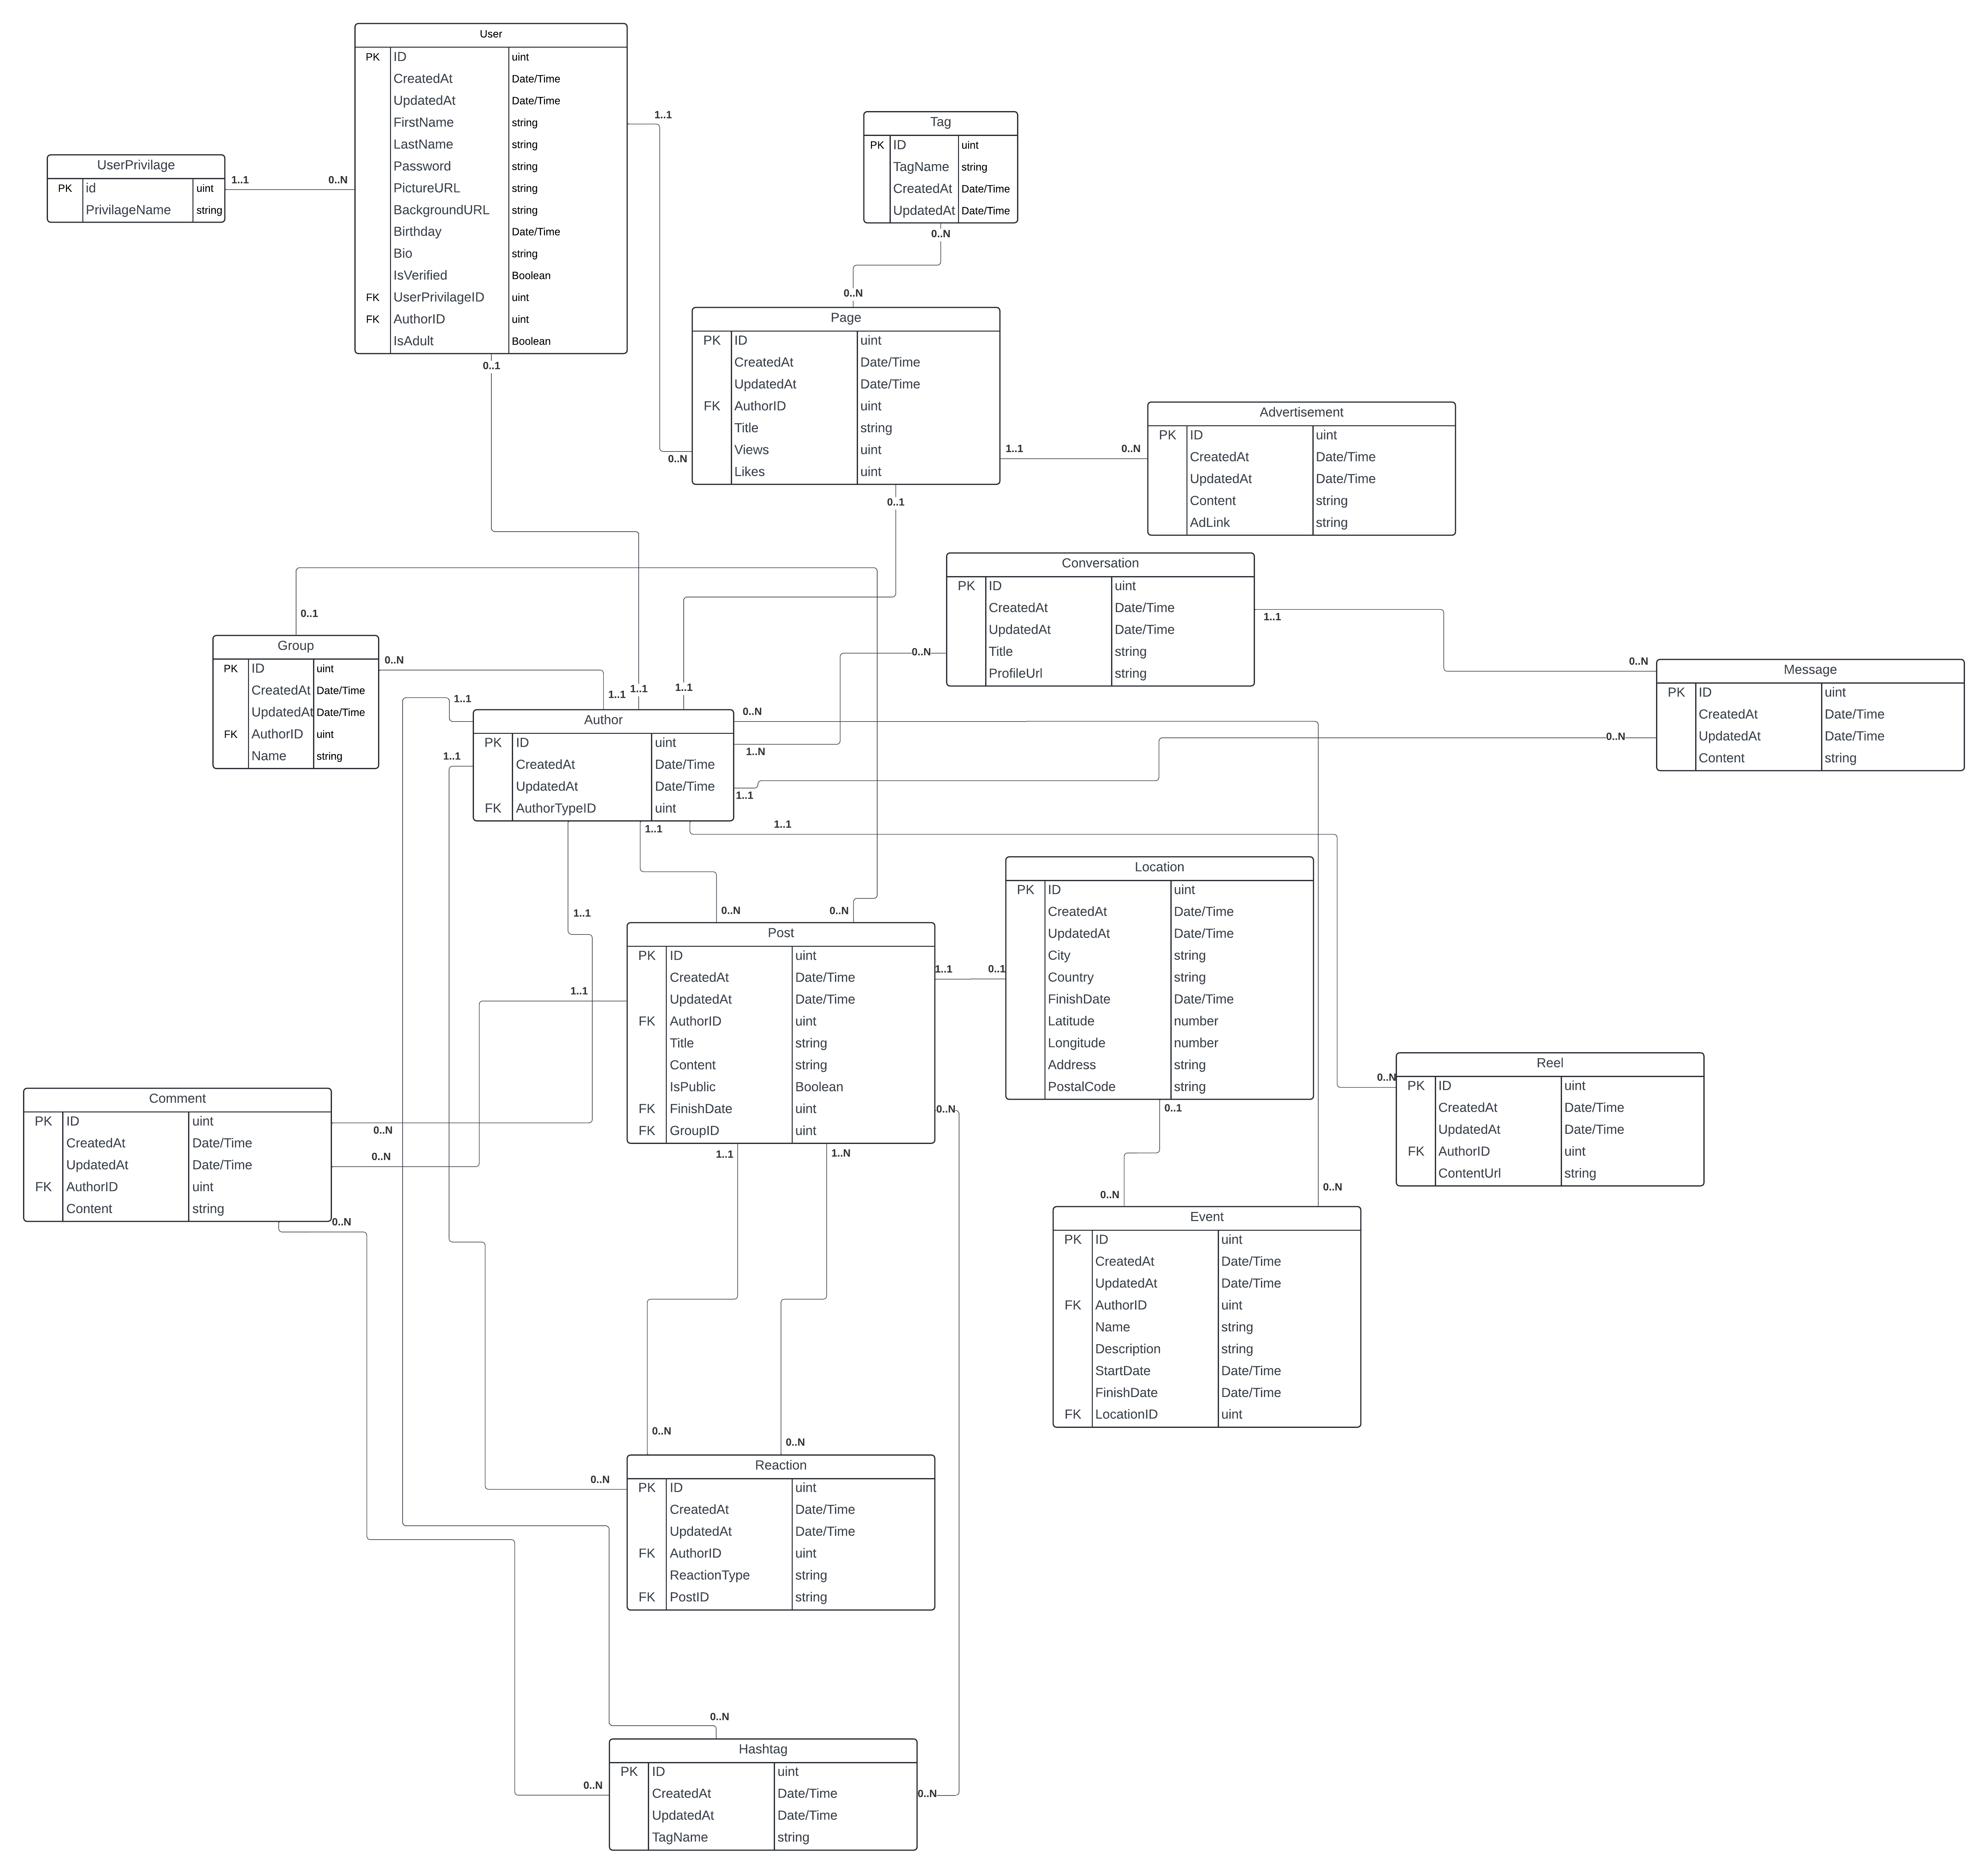
\includegraphics[width=\linewidth]{images/rel.png}
    \caption{Diagram relacji}
    \label{fig:rel}
\end{figure}

\section{Etap 3: Faza fizyczna}

Encje, które uległy zmianie:

\begin{itemize}
    \item Rozbicie lokalizacji na pomniejsze tabele
    \item Zamiana na enumy: typu autora oraz statusu zaproszenia do znajomych
    \item Dodanie do encji Conversation pole Members, które przechowuje id użytkowników biorących udział w konwersacji
\end{itemize}


Wykorzystano instrukcję CHECK do potwierdzenia poprawności danych w paru encjach. Przykładowo:
\begin{itemize}
    \item 'A' nie moze być przyjacielem 'A'
    \item 'A' nie moze wysłać zaproszenia do znajomych do 'A'
    \item Czas rozpoczęcia wydarzenia musi być wcześniejszy niż czas zakończenia wydarzenia
    \item Grupa musi mieć od 1 do 10000000 członków.
\end{itemize}

Do stworzenia struktury bazy wykorzystano mechanizm ORM - (\href{https://gorm.io/}{gorm}). Sama baza wymagała dopracowania jeśli chodzi o enumeracje oraz reguły usuwania już bezpośrednio w systemie PostgreSQL (pgadmin).

\textbf{Usuwanie}: Każdy model posiada pole \textit{DeletedAt} z indeksem. Podczas usuwania danego wiersza pole \textit{DeletedAt} jest ustawiane na znacznik czasu (timestamp) wskazujący moment, w którym dane zostały usunięte. Dzięki temu baza obsługuje soft deleting. Oznacza to, że gdy użytkownik usunie swoje konto, będzie można je przywrócić. Taką operację obsługują na przykład serwisy takie jak Facebook.

\begin{figure}[H]
    \centering
    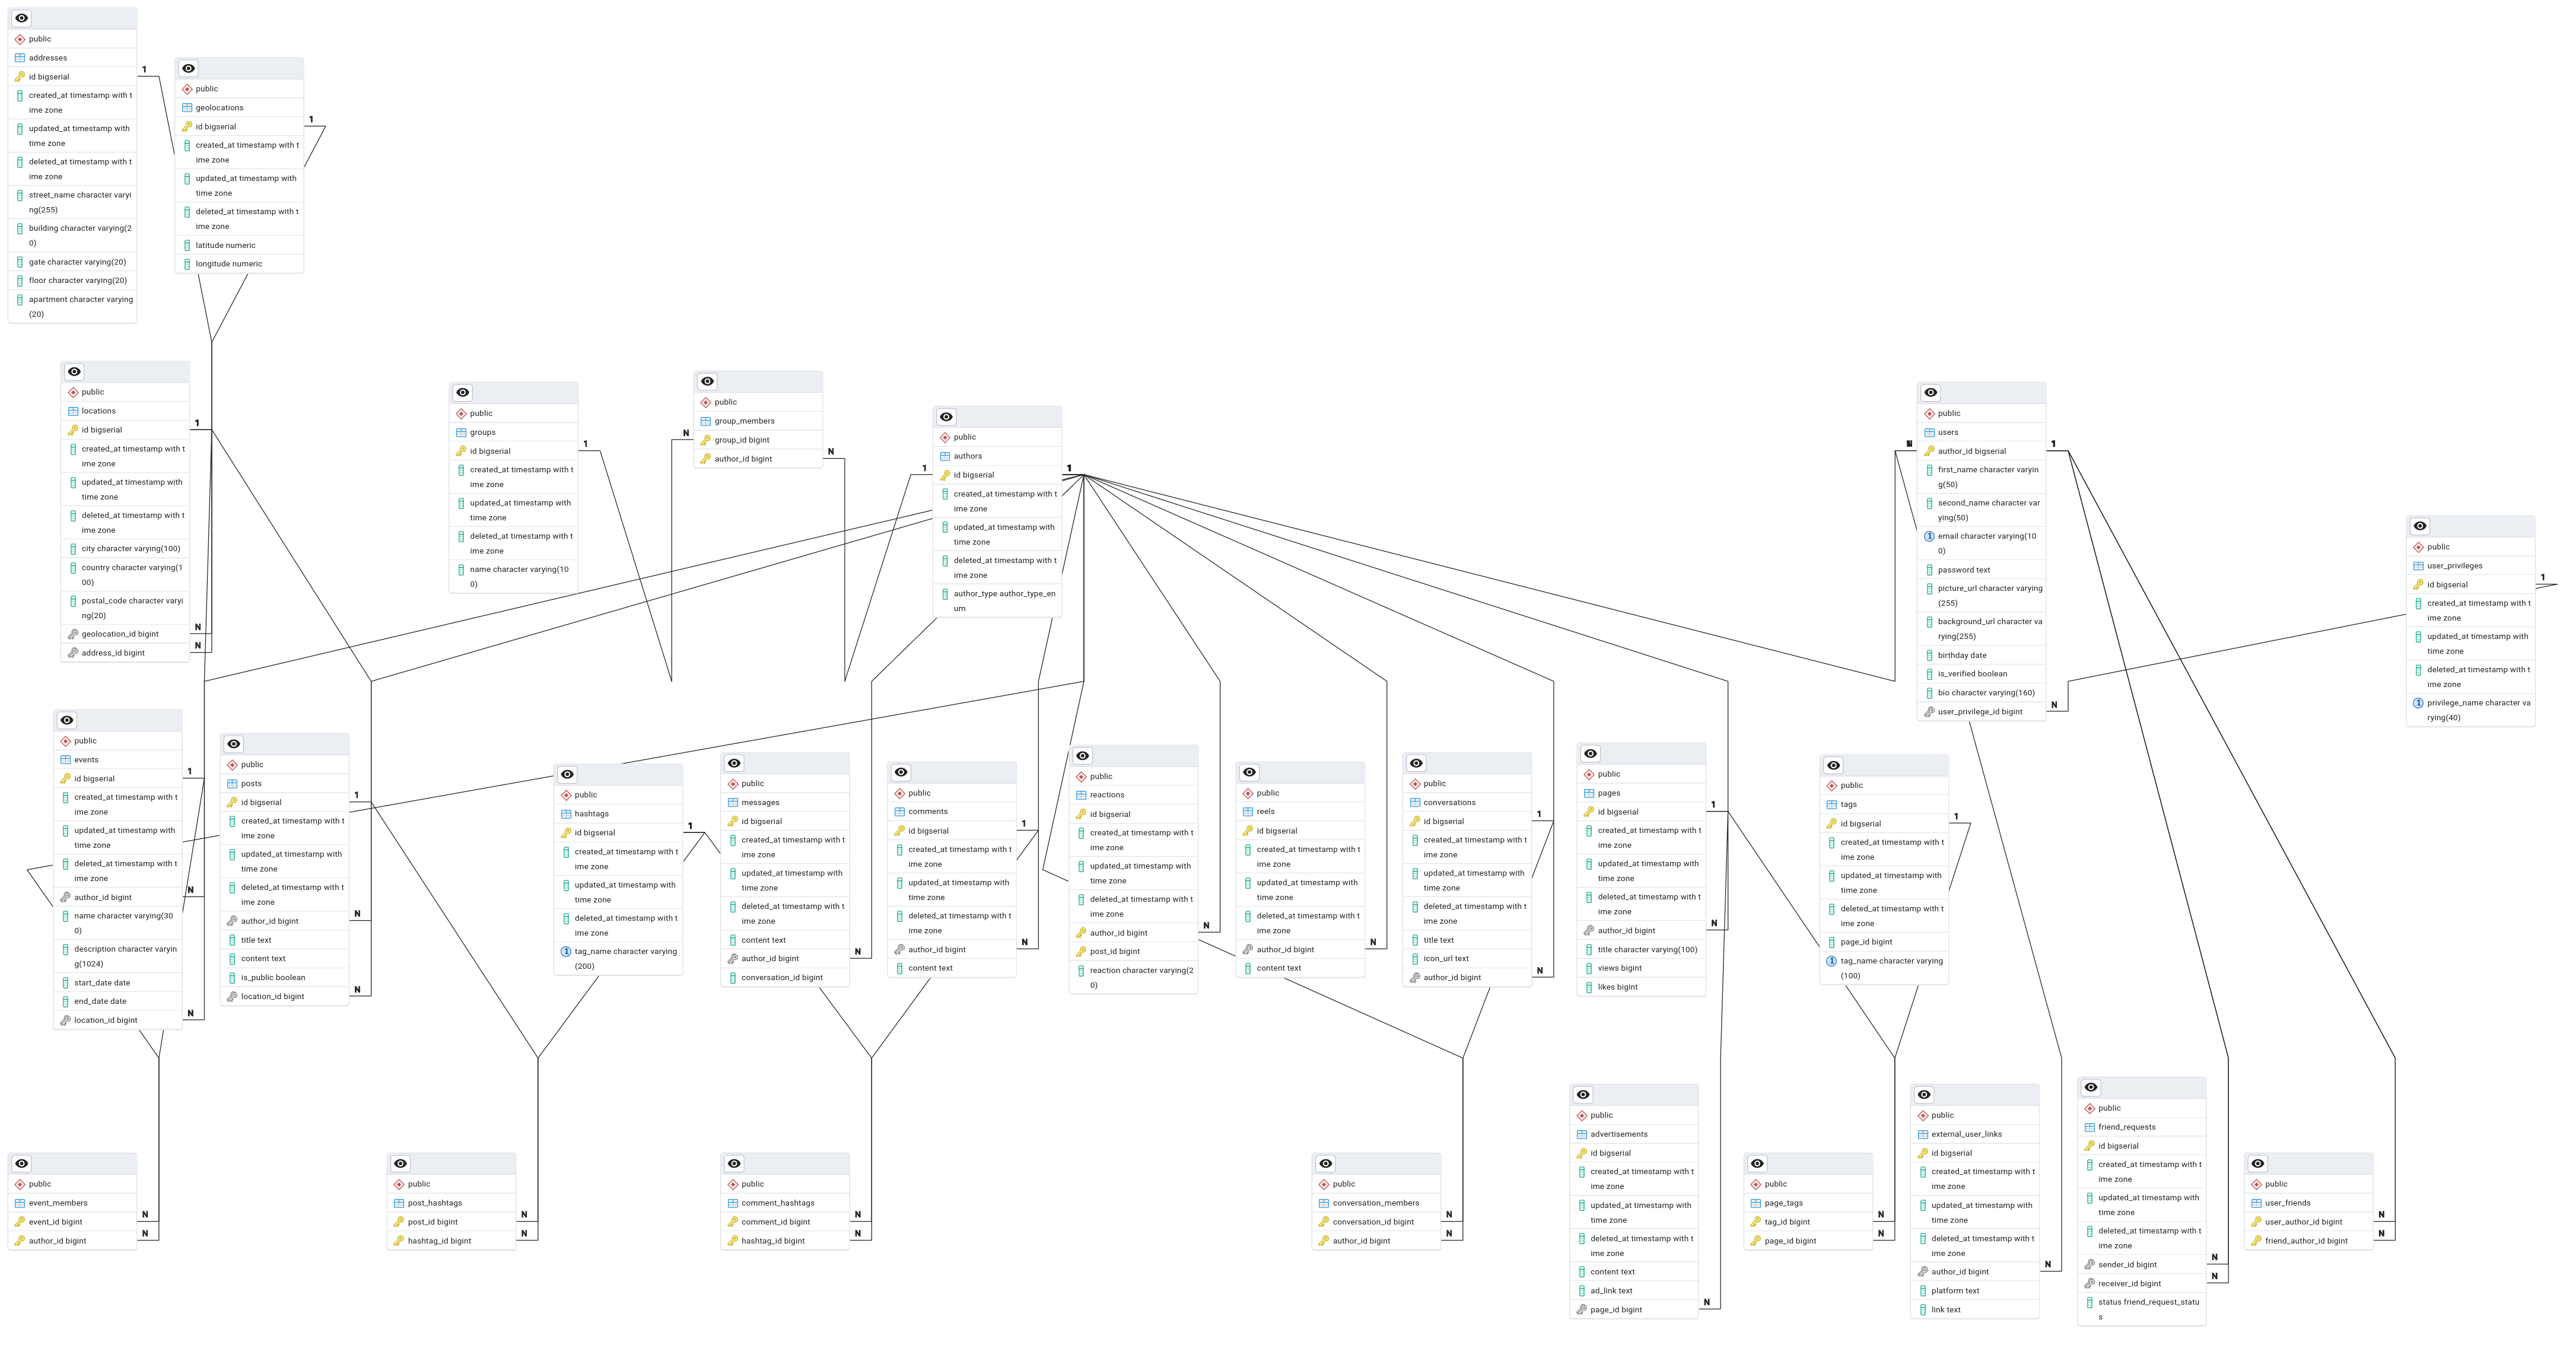
\includegraphics[width=\linewidth]{images/postgres_diagram.png}
    \caption{Diagram relacji z PostgreSQL}
    \label{fig:postgres}
\end{figure}


\section{Etap 4: Faza fizyczna 2}

\quad Standardowo kod można zobaczyć w repozytorium na gicie: \href{https://github.com/lukaszfabia/social_media_db}{social media db}. \\

\quad Mając napisany ORM poprzenio, w tym etapie pozostało napisać funkcje generujące dane do bazy. Rozwiązanie można podzielić na 3 cześci (od szczegółu do ogółu):

\begin{enumerate}
    \item Dekorator, który będzie wykonywać okreśolny blok \texttt{count} razy.
    \item Funkcja, generująca dany typ danych np. generator użytkowników.
    \item Odpowienie ułożenie wywołań.
\end{enumerate}

Zapełnianie bazy danych dużą ilością danych zajmuje stosunkowo dużo czasu, może to być spowodowane przez unikalność niektórych atrybutów(biblioteka "męczy" się z generowaniem unikalnych sensownych danych), ale także przez wywołania które tworzą listy autorów dla np. eventów, ostatnim podejrzeniem może być nieoptymalnie napisany kod. \\


\textbf{Język}: \href{https://go.dev/}{Go}

\textbf{Generowanie sztucznych danych}: \href{https://github.com/brianvoe/gofakeit}{gofakeit}

\textbf{Object relational mapping (ORM)}: \href{https://github.com/go-gorm/gorm}{gorm} \\

Reszta rzeczy, które zostały wykonane:

\begin{itemize}
    \item Funkcja usuwająca dane z tabel
    \item Własne implementacje niektórych danych np. \texttt{Title}, \texttt{Birthday}
    \item Konfiguracja loggera
    \item Funkcja haszująca hasło
\end{itemize}

\section{Etap 5: Faza fizyczna 3}

\quad W tej fazie projektu stworzyliśmy projekt interfejsu graficznego w programie Figma oraz napisaliśmy 10 nietrywialnych kwerend w SQL.

\subsection{Projekt interfejsu graficznego}
\quad Zaprojektowaliśmy następujące 10 widoków do aplikacji mobilnej:

\begin{itemize}
    \item Strona główna
    \item Strona komentarzy i rekacji
    \item Strona profilu
    \item Strona strony (page)
    \item Strona grupy
    \item Strona wydarzenia
    \item Strona konwersacji
    \item Strona panelu konwersacji
    \item Strona rolek (reel)
    \item Strona ze znajomymi
\end{itemize}

\quad Podczas projektowania zauważyliśmy parę drobnych rzeczy, które można by było poprawić - np. brak ikony czy grafiki tła dla strony. Tak więc poprawiliśmy takie nieścisłości i zaktualizowaliśmy kod seeder.go, który zajmuje się generowaniem tych danych.

\quad Pełny projekt interfejsu graficznego znajduje się w załączonym pliku "figma.pdf".

\begin{figure}[H]
    \centering
    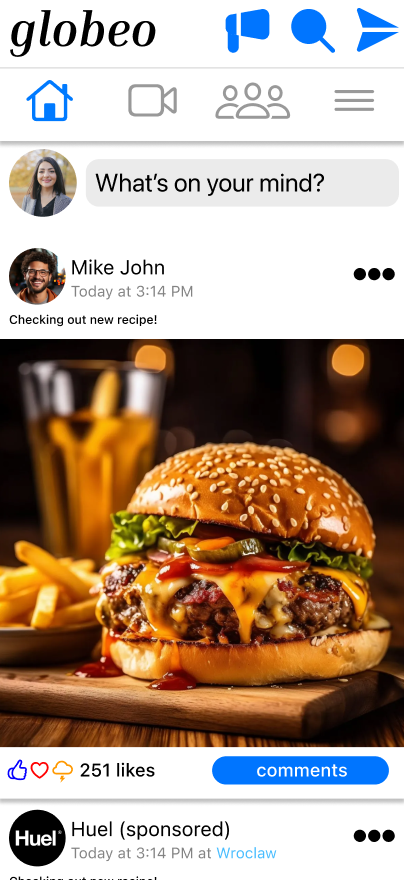
\includegraphics[width=0.25\textwidth]{images/figma.png}
    \caption{1 z widoków interfejsu graficznego}
    \label{fig:figma}
\end{figure}

\subsection{Kwerendy SQL}
\quad Poniżej znajdują się 10 kwerend SQL, które zostały napisane w celu przeszukania i stworzenia raportów na podstawie bazy danych:

\begin{itemize}
    \item 10 najpopularniejszych hashtagów z ostatnich 7 dni
    \item Konwersacje autora
    \item Publiczne posty autora
    \item Średnia liczba znajomych
    \item Średnia liczba poszczególnych reakcji na posty w ostatnim miesiącu
    \item Wydarzenia w danym mieście (np. Saint Petersburg)
    \item Wydarzenia, w których wezmą udział znajomi autora
    \item Tagi stron, posortowane po średniej liczbie polubień i wyświetleń
    \item Użytkownicy, z którymi użytkownik ma wspólnych znajomych
    \item Użytkownicy z najwiekszą średnią liczbą reakcji na posty
\end{itemize}

\begin{figure}[H]
    \centering
    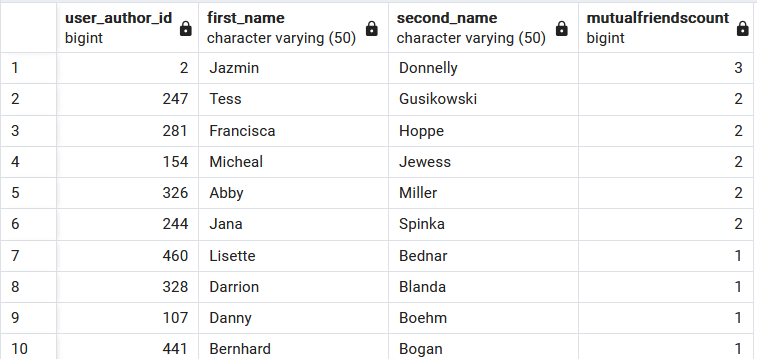
\includegraphics[width=\textwidth]{images/mutual_friends_sql.png}
    \caption{Wynik kwerendy wyszukującej użytkowników ze wspólnymi znajomymi}
    \label{fig:sql_1}
\end{figure}

\begin{figure}[H]
    \centering
    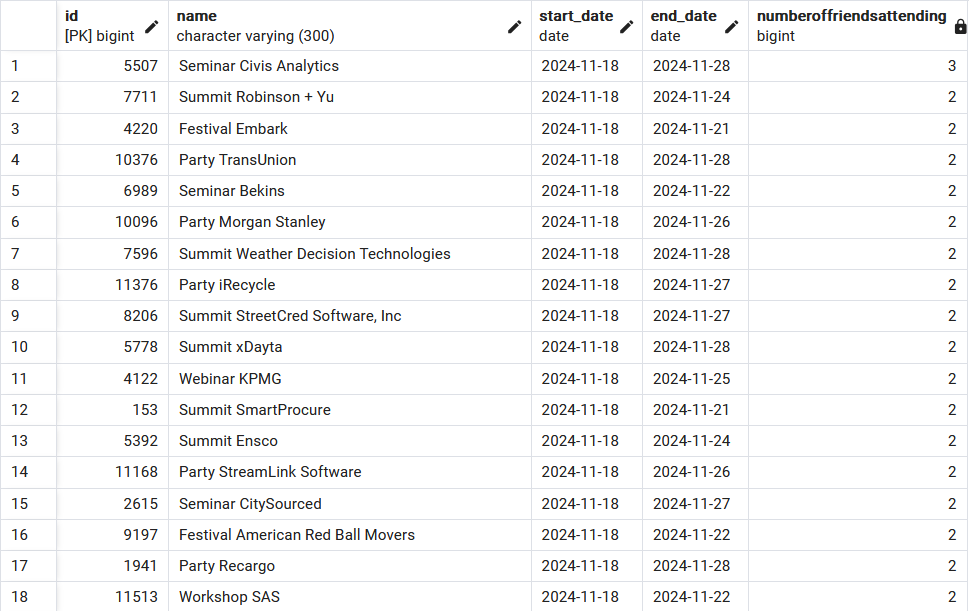
\includegraphics[width=0.7\textwidth]{images/event_mutuals_sql.png}
    \caption{Wynik kwerendy wyszukującej wydarzenia, na które zapisali się znajomi użytkownika}
    \label{fig:sql_2}
\end{figure}

\section{Etap 6: Faza fizyczna 4}

Przykładowy wynik działania \texttt{EXPLAIN}

\begin{verbatim}
    Seq Scan on foo  (cost=0.00..155.00 rows=10000 width=4)
\end{verbatim}

Ogólnie można powiedzieć, że komenda do dostarcza bardzo dokładne informacje w porównaniu np. do \textbf{MySQL}.\\

Powyższa komenda to sposób w jaki zapytanie może zostać wykonane. W tym wypadku mamy wykonanie sekwencyjne, czyli skanujemy całą tabelę w celu znalezienia wierszy spełniających warunki w kwerendzie.\\

\textbf{Koszt}(cost) - wartość po lewej to koszt początkowy zapytania tutaj jest on równy 0.00, kolejna wartość to szacowany koszt operacji, wartość ta jest obliczana przez system bazodanowy.

\textbf{Wiersze}(rows) - ilość wierszy spełniająca dane kryteria.

\textbf{Szerokość}(width) - waga wiersza w \underline{bajtach}\\

Zatem optymalizacja zapytań będzie polegała na minimalizacji tych "kosztów". W tym celu wykorzystuje się \textbf{indeksy}. \\

\subsection{Różne typy indeksów i ich zastosowanie}

\begin{table}[htbp]
    \begin{tabular}{|l|l|}
        \hline
        \multicolumn{1}{|c|}{\textbf{Typ indeksu}} & \textbf{Zastosowanie}                                               \\ \hline
        \textbf{B-Tree}                            & Wyszukiwanie, sortowanie, zakresy, klucze główne, indeksy unikalne. \\ \hline
        \textbf{Hash}                              & Szybkie porównania równości (=).                                    \\ \hline
        \textbf{GiST}                              & Dane przestrzenne, zakresy, hierarchie.                             \\ \hline
        \textbf{BRIN}                              & Duże tabele z posortowanymi danymi, dane archiwalne.                \\ \hline
    \end{tabular}
\end{table}


\newpage

\subsection{Obserwacje}

Indeksy nie pomogą w każdej operacji - na przykład dla kwerend, gdzie największym kosztem jest grupowanie, mogą niekoniecznie pomóc.

Hash nie przynosi znaczącej poprawy wydajności w naszych zapytaniach w porównaniu z B-tree.

Zapytania wykorzystujące funkcje agregujące są trudne do optymalizacji, a dodanie indeksów w większości przypadków nie przyniosło zauważalnych korzyści.

Wyjątek stanowi zapytanie \textbf{show\_events\_in\_st\_petersburg}, gdzie zastosowanie indeksu złożonego przyniosło wyraźną poprawę:
\begin{itemize}
    \item Zastosowanie indeksu typu \textbf{B-tree} zmniejszyło koszt zapytania o około 10\%.
    \item Dodanie indeksu typu \textbf{BRIN} dodatkowo obniżyło koszt o kolejne 10\%.
\end{itemize}

Dla zapytań niewykorzystujących funkcji agregujących, dodanie indeksów pozwoliło na kilkukrotne zmniejszenie kosztów ich wykonania.


\begin{figure}[htbp]
    \centering
    \begin{minipage}{0.45\textwidth}
        \centering
        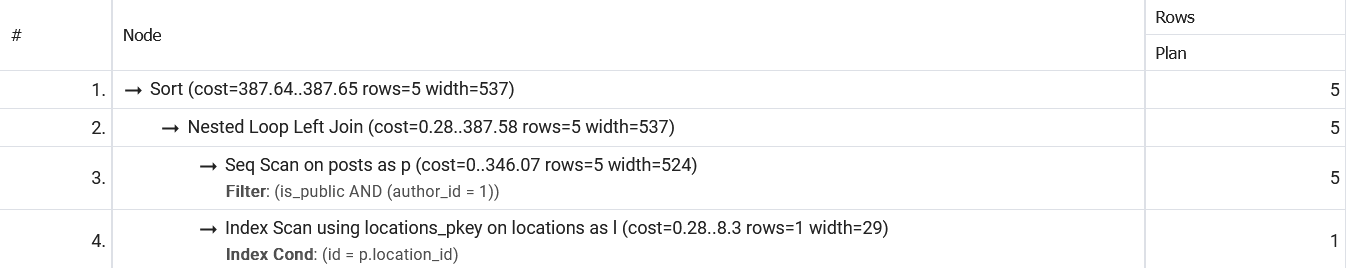
\includegraphics[width=\linewidth]{images/index_show_authors_posts_before.png}
        \label{fig:index_show_authors_posts_before}
    \end{minipage}
    \hfill
    \begin{minipage}{0.45\textwidth}
        \centering
        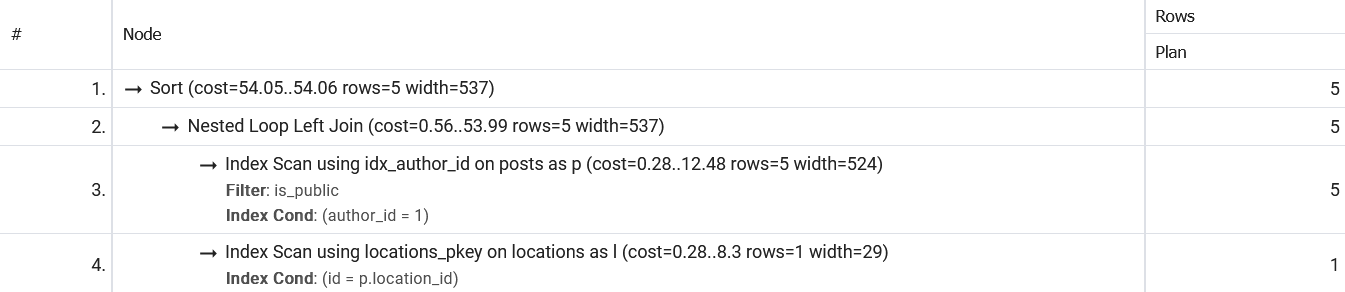
\includegraphics[width=\linewidth]{images/index_show_authors_posts_after.png}
        \label{fig:index_show_authors_posts_after}
    \end{minipage}
    \caption{Przykładowe czasy zapytań bez i z indeksami.}
\end{figure}

\begin{figure}[htbp]
    \centering
    \begin{minipage}{0.45\textwidth}
        \centering
        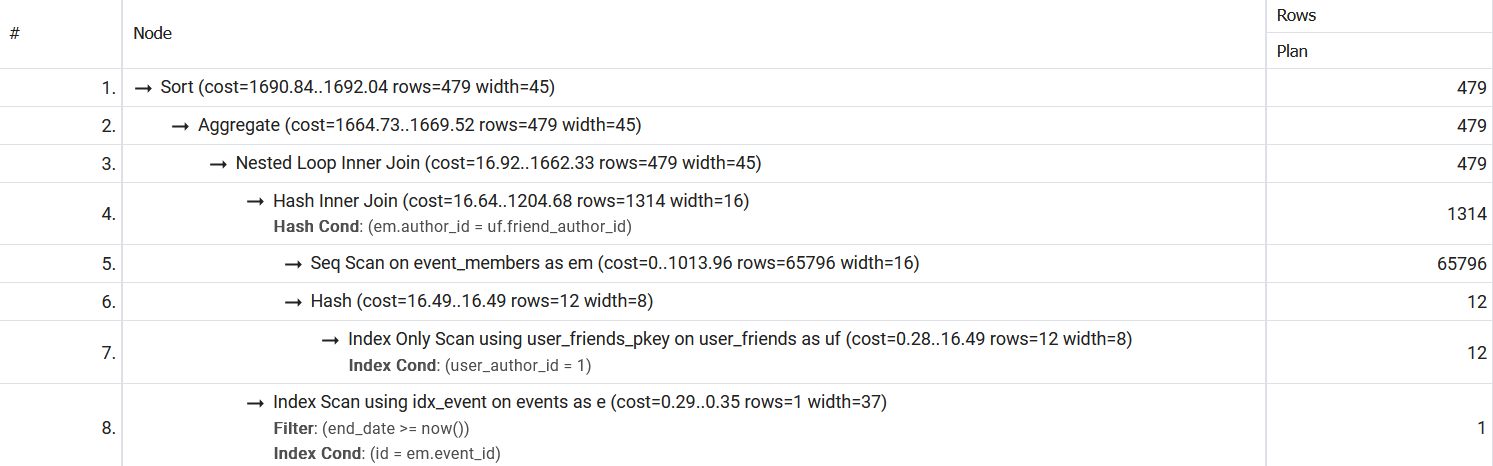
\includegraphics[width=\linewidth]{images/index_show_events_with_friends_before.png}
        \label{fig:index_show_events_with_friends_before}
    \end{minipage}
    \hfill
    \begin{minipage}{0.45\textwidth}
        \centering
        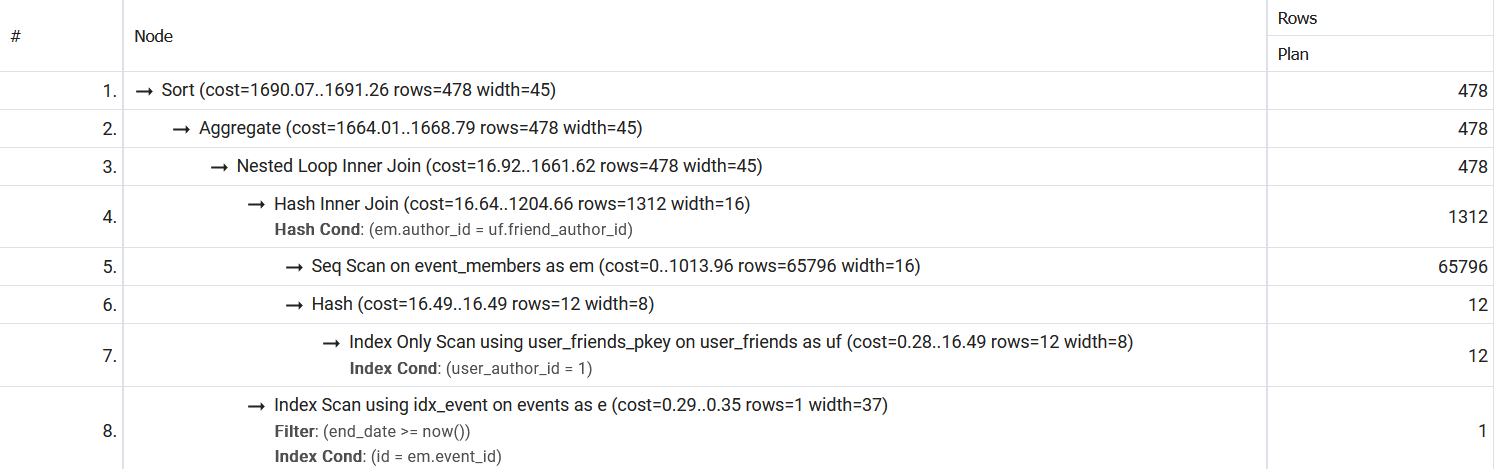
\includegraphics[width=\linewidth]{images/index_show_events_with_friends_after.png}
        \label{fig:index_show_events_with_friends_after}
    \end{minipage}
    \caption{Przykładowe czasy zapytań bez i z indeksami.}
\end{figure}


\begin{figure}[htbp]
    \centering
    \begin{minipage}{0.3\textwidth}
        \centering
        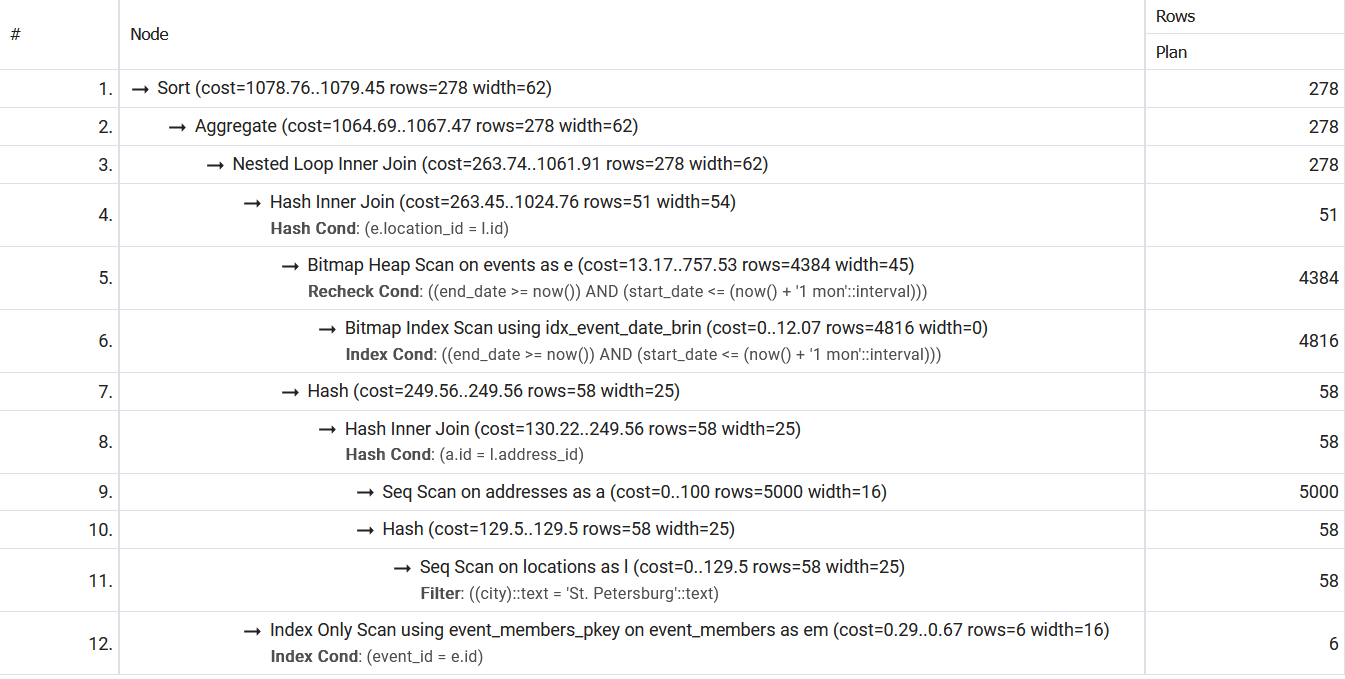
\includegraphics[width=\linewidth]{images/show_events_in_st_petersburg with composite index (end_date, start_date) using brin.png}
        \label{fig:show_events_in_st_petersburg1}
    \end{minipage}
    \hfill
    \begin{minipage}{0.3\textwidth}
        \centering
        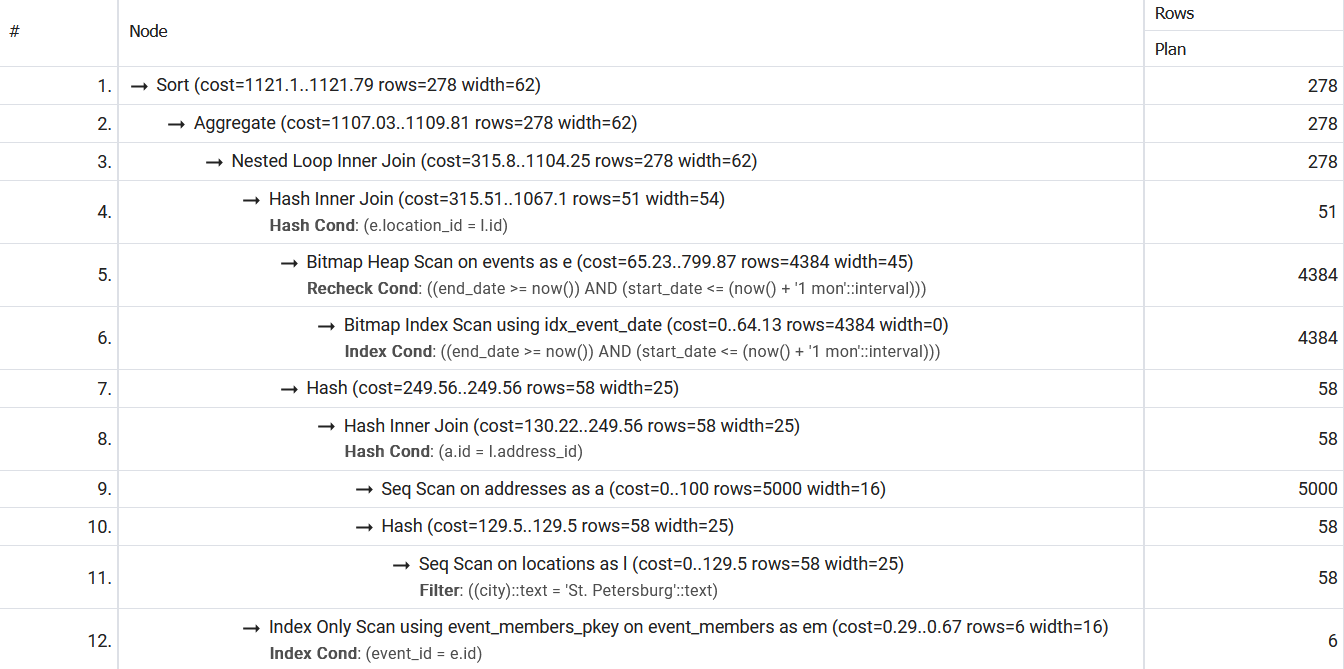
\includegraphics[width=\linewidth]{images/show_events_in_st_petersburg with composite index (end_date, start_date).png}
        \label{fig:show_events_in_st_petersburg3}
    \end{minipage}
    \hfill
    \begin{minipage}{0.3\textwidth}
        \centering
        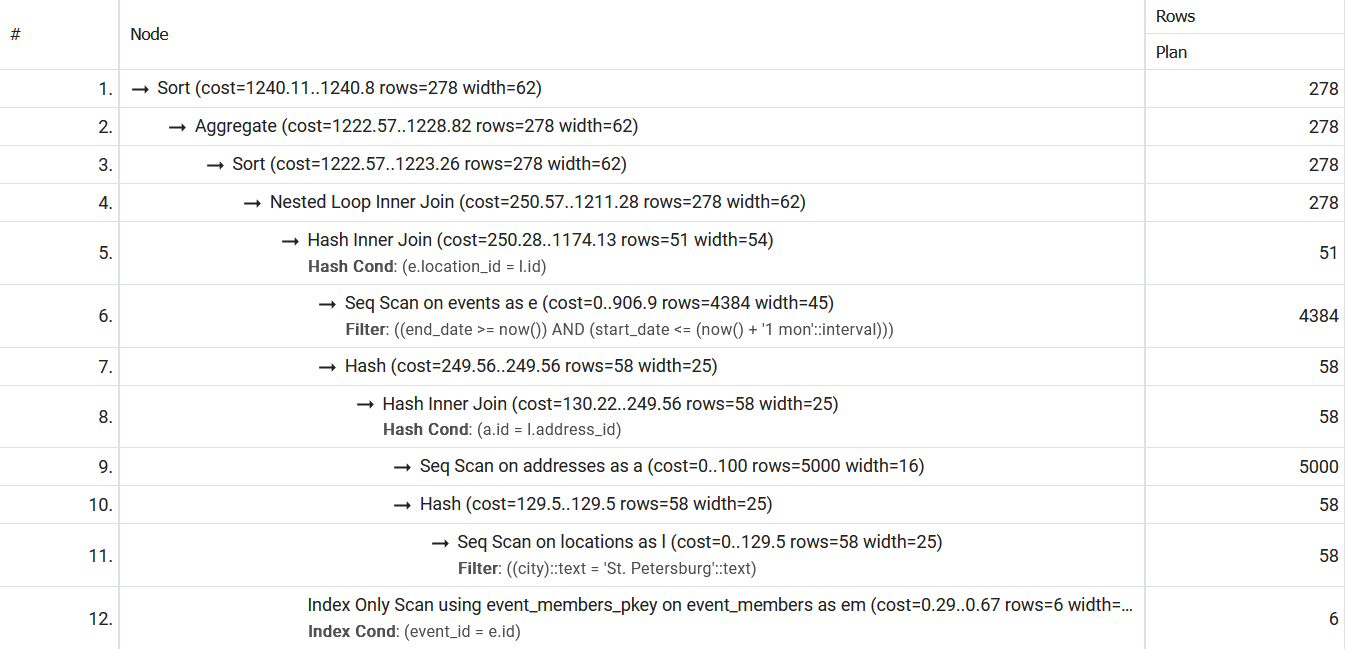
\includegraphics[width=\linewidth]{images/show_events_in_st_petersburg without composite index.png}
        \label{fig:show_events_in_st_petersburg2}
    \end{minipage}
    \caption{Optymalizacja zapytania z wydarzeniami w Piotrogrodzie}
\end{figure}

\newpage

\section{Etap 7: Faza fizyczna 5}

\subsection{Sprawozdanie powykonawcze}

\subsubsection{Mocne strony projektu (S)}


Jedną z pierwszych mocnych stron projektu jest wydzielenie tabeli \texttt{authors}. Pozwoliło to na rozszerzenie możliwości tworzenia nowych tabel dla użytkowników (\texttt{user}, \texttt{page}). Dodatkowo w ten sposób pozbyto się \textit{redundantnych} relacji, ponieważ zarówno \textbf{strona}, jak i \textbf{użytkownik} mogli w domyśle wykonywać te same czynności na innych tabelach.

Zastosowanie usuwania kaskadowego również okazało się być bardzo pomocne, ponieważ w ten sposób przy usuwaniu jakichkolwiek danych mielibyśmy pewność, że dane pozostaną spójne.

Będąc w temacie usuwania, dane z bazy nie były całkowicie usuwane(\textit{hard delete}). To nie tylko pozwoliłoby na przywrócenie danych, na przykład konta niezdecydowanego użytkownika, ale również pozwoliłoby śledzić historię danych. Ponadto dane, które nie są widoczne dla użytkonika mogą posłużyć np. do analiz biznesowych.

Uzyskanie zgodności z przepisami, w tym z RODO w naszym projekcie wydaje się ułatwione przez dwa czynniki:
\begin{itemize}
    \item Haszowanie haseł
    \item Wydzielenie danych osobowych do osobnej tabeli, dzięki czemu można łatwo zarządzać dostępem do tych danych, a także przeprowadzić \textit{soft delete} użytkownika bez usuwania wszystkich rzeczy, które wytworzył.
    \item Usuwanie kaskadowe, które pozwala na szybkie usunięcie wszystkich danych związanych z użytkownikiem.
    \item Ograniczenie zbieranych danych do niezbędnych, co pozwala na zminimalizowanie ryzyka naruszenia RODO.
\end{itemize}

Skrypt generujący dane również jest mocną stroną projektu. Skrypt generuje tabele w bazie danych, dodając potrzebne ograniczenia do atrybutów, enumeracje oraz dość sensowne dane. Jest on solidną bazą pod część backendową (związaną z warstwą modeli np. dla \textit{architektury warstwowej}) aplikacji. Dodatkowym atutem jest to, że generacja danych nie jest destruktywna - mając już dane w bazie danych, możemy spokojnie wywołać metodę odpowiedzialną za generowanie dodatkowych danych w określonych przez nas tabelach.

Dodatkowo można w prosty sposób zmienić system, dla którego ma być generowana baza - my korzystaliśmy z PostgreSQL, ale bez większych problemów dałoby się zmienić system na inny (na przykład SQLite, MySQL czy SQLServer) dzięki używaniu GORM'a, który jest właśnie kompatybilny z wieloma systemami.

Został napisany również skrpty, który automatycznie uruchomi bazę w kontenerze \texttt{Dockerowym}, dzięki czemu nie trzeba instalować samego PostgreSQL, PGAdmin czy innych pluginów, żeby zarządzać tą bazą - wystarczy podać parę podstawowych danych w pliku \texttt{.env} i uruchomić skrypt. Dodatkową zaletą jest to, że baza jest uruchamiana w izolowanym środowisku, co pozwala na łatwe testowanie różnych wersji bazy danych, a także na łatwe przenoszenie bazy na inne środowisko (np. z lokalnego na serwer produkcyjny).

Dodatkową automatyzacją jest integracja backendu z komendami umieszczonymi w Makefile'u. Dzięki temu można w prosty sposób uruchomić skrypt generujący dane, uruchomić bazę danych, przeczyścić bazę i inne.

Co do wybranego systemu, system PostgreSQL, okazał się on być całkiem wydajnym pod względem operacji typu \textit{CRUD} na tabelach. Dzięki dodaniu indeksów, kwerendy zostały jeszcze bardziej zoptymalizowane.

Wydaje nam się, że dzięki uogólnieniu wszystkich czatów do grupowych (czat 1-1 nie różni się formalnie od czatu wieloosobowego w naszej bazie) zmniejszamy ryzyko błędów przez utrzymywanie dwóch wersji konwersacji. Nie powinno to sprawić nam problemów implementacyjnych w przyszłości, a dodatkowo dodanie lub usunięcie użytkownika z konwersacji będzie bardzo proste.

Nasz projekt stara się oczywiście spełniać podstawowe założenia dobrej bazy danych - jest spójny, niepowtarzalny, znormalizowany, a także ma ograniczenia integralnościowe. Żadne dane nie występują niepotrzebnie więcej niż raz. Encje wydają się być dobrze znormalizowane. Ograniczenia integralnościowe są zaimplementowane w postaci kluczy obcych, ograniczeń CHECK oraz unikalności. Wszędzie, gdzie to miało sens, wprowadziliśmy tabele asocjacyjne, aby uniknąć problemów związanych z relacjami wieloma do wielu - udało się je wszystkie usunąć z naszego projektu.


\subsubsection{Słabe strony projektu (W)}

Największą słabą stroną projektu jest dość wolno działający skrypt generujący dane. Dzieje się tak, gdy chcemy dodać więcej wierszy do tabeli - przez to, że skrypt wybiera foreign keys losowo wśród istniejących już elementów, często jest duża szansa niepowodzenia przez złamanie jakiejś zasady - dałoby się to ulepszyć dzięki bardziej inteligentemu wybieraniu foreign keys. Wygenerowanie niektórych danych wymaga też skomplikowanej i zagnieżdżonej logiki tworzenia elementów. Być może problemem jest też biblioteka \textit{faker}, która nie bardzo radziła sobie z generowaniem bardzo losowych, często unikalnych danych.

Okazuje się, że draw.io (narzędzie do modelowania diagrmów, w naszym wypadku diagramów ERD) ma wbudowaną integrację z GORM'em, dzięki której wystarczyłoby przesunąć diagram nad okienko z kodem. Ostatecznie nie oszczędziłoby nam to dużo czasu, ale z pewnością ułatwiłoby pracę i zmniejszyłoby ryzyko literówek.

\subsubsection{Możliwości (O)}

Tak jak już wcześniej wspominaliśmy, baza jest dobrą podstawą do stworzenia systemu na wzór \textbf{Facebooka} czy \textbf{Twittera/X} poprzez zbudowanie jakiegoś prostego serwisu REST'owego. Dzięki temu, że serwis byłby faktycznie używany na większą skalę, zauważylibyśmy więcej problemów optymalizacyjnych. Pozwoliłoby to na dopracowanie bazy danych w miejscach, gdzie brakowałoby wydajności.

Jeśli chodzi o możliwości rozbudowy bazy to można by dodać np. lepszą obsługę mediów (wydzielenie osobnej tabeli). Można być też poprawić tabele związane z lokalizacjami i zamiast przechowywania danych koordynatów przechowywać typ \texttt{Point} do obsługi współrzędnych geograficznych wykorzystując plugin \textbf{PostGIS}. Można by wtedy ulepszyć sposób wyszukiwania wydarzeń użytkownikowi, poprzez szukanie ich w promieniu \textit{n} m/km od wybranego punktu.

\subsubsection{Zagrożenia (T)}

Problemem baz relacyjnych jest trudność w horyzontalnym skalowaniu, ponieważ zapewnienie spójności danych i transakcyjności (ACID) w rozproszonej architekturze jest skomplikowane. Tradycyjnie łatwiej jest skalować je pionowo, czyli ulepszać pojedynczą maszynę, dodając więcej zasobów, takich jak pamięć RAM, mocniejszy procesor czy szybsze dyski. Jednak przy zastosowaniu odpowiednich technik, takich jak sharding czy replikacja, możliwe jest również skalowanie horyzontalne baz relacyjnych. Tabela, która może być problematyczna w utrzymaniu to, na przykład, tabela z wiadomościami, które użytkownicy wysyłają sobie wzajemnie.  W przypadku tabeli z wiadomościami może to być problem, ponieważ może ona gwałtownie rosnąć. Dlatego lepszym rozwiązaniem byłoby podejście hybrydowe - przeniesienie niektórych tabel do baz NOSQL, dzięki czemu można by rozproszyć obliczenia, a nasz system nie miałby problemów z powolnym przeszukiwaniem bazy.

Baza wymagałaby też dużo optymalizacji, by wspierać miliony użytkowników stabilnie - aktualnie ciężko powiedzieć, jak dobrze by sobie radziła w takiej sytuacji - można by wprowadzać więcej indeksów które najlepiej radzą sobie z konkretną sytuacją, ale ciężko powiedzieć, czy to by wystarczyło.

\subsubsection{Podsumowanie}

Próbując wprowadzić produkt z taką bazą danych w życie, mielibyśmy wielki problem z konkurencją - Facebook, Twitter, Instagram, TikTok, LinkedIn, Pinterest, Reddit, Snapchat, Tumblr, WhatsApp, YouTube, czyli największe platformy społecznościowe, mają już swoje miejsce na rynku. Nasz produkt musiałby być bardzo innowacyjny, aby przyciągnąć użytkowników.

Jednakże, nasz projekt jest dobrym punktem wyjścia do stworzenia takiego produktu. Baza danych jest solidna, choć wymagałaby jeszcze sporo optymalizacji. Skrypt generujący dane jest bardzo pomocny do debuggowania i byłby krytycznie potrzebny tworząc MVP, ale wymagałby jeszcze sporo pracy, aby działał szybciej i bardziej efektywnie.

Czym mógłby wyróżniać się potencjalny produkt oparty na naszej bazie danych? Dobrym punktem wyjścia jest to, że nasza baza jest dość generyczna - większość wcześniej wymienionych serwisów ma już podobne encje. Tak więc można by rozwinąć tą bazę w jednym z tych 4 przykładowych kierunków:

\begin{itemize}
    \item \textbf{Baza danych dla GoLocal} - aplikacja do tworzenia i głosowania na wydarzenia dla samorządów i zwykłych ludzi, aplikacja w formie serwisu społecznościowego. Dodanie obsługi ankiet, opinii użytkowników o wydarzeniu, rozwinięcie tabel z lokalizacjami oraz wydarzeniami, obsługa użytkowników \textit{premium}. Usprawnienie obsługi komunikacji między użytkownikami, połączenie serwera z bazą NOSQL do zarządzania wiadomościami. W dalekiej przyszłości możnaby zastanowić się nad dedykowaną bazą do obsługi systemu rekomendacji - hurtowanie danych historycznych (usuniętych profili, rekacji, wydarzeń, postów, komentarzy).
    \item \textbf{Baza danych dla serwisu społecznościowego dla programistów} - dodanie tabeli związanej z projektami, repozytoriami, commitami, pull requestami, itd. Można by też dodać tabelę związane z technologiami, językami programowania, frameworkami, itd.
    \item \textbf{Baza danych dla serwisu społecznościowego dla naukowców} - dodanie tabeli związanej z publikacjami, konferencjami, grantami, itd. Można by też dodać tabelę związane z dziedzinami nauki, konferencjami, itd.
    \item \textbf{Lepszy Twitter} - przez ostatnie zamieszanie w serwisie Twitter/X, można by stworzyć serwis, który byłby bardziej przejrzysty, miałby lepsze algorytmy rekomendacji, byłby bardziej stabilny i bardziej moderowany, itd.
\end{itemize}

\subsection{Wprowadzone modyfikacje}

\subsubsection{Porzucone pomysły}
Już w początkowej fazie tworzenia projektu doszliśmy do wniosku że opcja zgłaszania postów/treści przez użytkowników wymaga nieadekwatnego nakładu pracy w stosunku do korzyści jakie nasz projekt na tym etapie mógłby z tego zyskać. Może być to dobra funkcjonalność do dodania w ramach rozwoju aplikacji, jednak na początkowych etapach stwierdziliśmy, że postawimy na jakość, a nie ilość. Dlatego zrezygnowaliśmy z tego pomysłu, aby w pełni skupić się na pozostałych funkcjonalnościach.
Podobnie stało się z encją “Story”. Jako że jej atrybuty praktycznie nie różniłyby się od obecnych już encji (Post, Reel) zdecydowaliśmy się na jej pominięcie w późniejszych etapach projektu. Jednak tak jak w przypadku zgłaszania postów jest to jak najbardziej funkcjonalność możliwa do dodania w przyszłości, a dzięki podobieństwu do obecnych już encji wdrożenie Story do naszej bazy danych powinno być nawet prostsze niż dodanie opcji zgłaszania postów.


\subsubsection{Nowe encje}
Na pierwszym diagramie ERD naszego projektu nie uwzględniliśmy encji “Tag”, która została dodana w następnym etapie. Encja ta określa typ prowadzonej strony. Nie uwzględniliśmy również encji “UserPrivilege”, która została dodana dopiero w fazie logicznej. Zdecydowaliśmy się wyodrębnić User Privilege do osobnej encji zamiast używać enuma, aby ułatwić modyfikację czy rozbudowę bazy danych oraz zmniejszyć ryzyko niespójności.
Pojawiła się też encja “ExternalAuthorLinks” która pozwala przechowywać linki do innych social mediów użytkownika.


\subsubsection{Rozdzielenie lokacji na 3 table}
Encja związana z lokacją została rozdzielona na 3 osobne encje: Location, Geolocation, Address. Taka struktura danych niweluje powielanie informacji, ponieważ miasta, kody pocztowe czy nawet współrzędne geograficzne mogą być takie same dla wielu adresów. Dodatkowo możemy teraz w bardzo precyzyjny sposób określić adres, do jakiego się odwołujemy -  mamy możliwość sprecyzowania ulicy, budynku, klatki schodowej, piętra i mieszkania. Dzięki temu, niezależnie od konwencji zapisu adresu (które mogą się różnić w zależności od kraju) użytkownik będzie w stanie wprowadzić go do naszej bazy danych.
Poza tym rozdzielenie lokacji na osobne encje zmniejsza ryzyko niespójności, ułatwia modyfikacje i rozszerzanie bazy danych oraz sprawia, że zapytania na tabeli Location są bardziej wydajne. Jako że atrybuty tej encji zostały ograniczone do minimum, a bardziej złożone dane przechowywane są w osobnych tabelach, podczas wykonywania na przykład zapytań dotyczących wydarzeń w danym mieście nie potrzebujemy importować danych ze wszystkich tabel - wystarczy nam sama tabela Location co zwiększa wydajność zapytań.


\section{Etap 8: Faza logiczna I}

\subsection{Update ERD'a}

Diagram ERD \ref{fig:new_erd} został zaktualizowany - odzwierciedla schemat relacji w bazie oraz jest czytelniejszy względem poprzedniego. Zdecydowaliśmy się nie umieszczać szczątkowych artybutów dla encji, ponieważ wprowadziło by to zbędne zamieszanie i wpłyneło by to na czytelność.

Zmieniono:

\begin{itemize}
    \item Dodano \texttt{User Privilege}
    \item Rozbito \texttt{Location}, na pomniejsze encje (Address, Geolocation)
    \item Wyodrębniono nową encje \texttt{Tag}
    \item Usunięto encje \texttt{Story}
    \item Pokazaliśmy na diagramie relacje użytkownika z innymi użytkownikami (asocjacja \textit{likes (as buddy)}) oraz podobnie pokazaliśmy wysyłanie zaproszeń do znajomych (asocjacji \textit{receives}, \textit{sends}).
    \item No i usuneliśmy encje \texttt{Process}, dodaną przypadkiem.
\end{itemize}


\begin{figure}[htbp]
    \begin{center}
        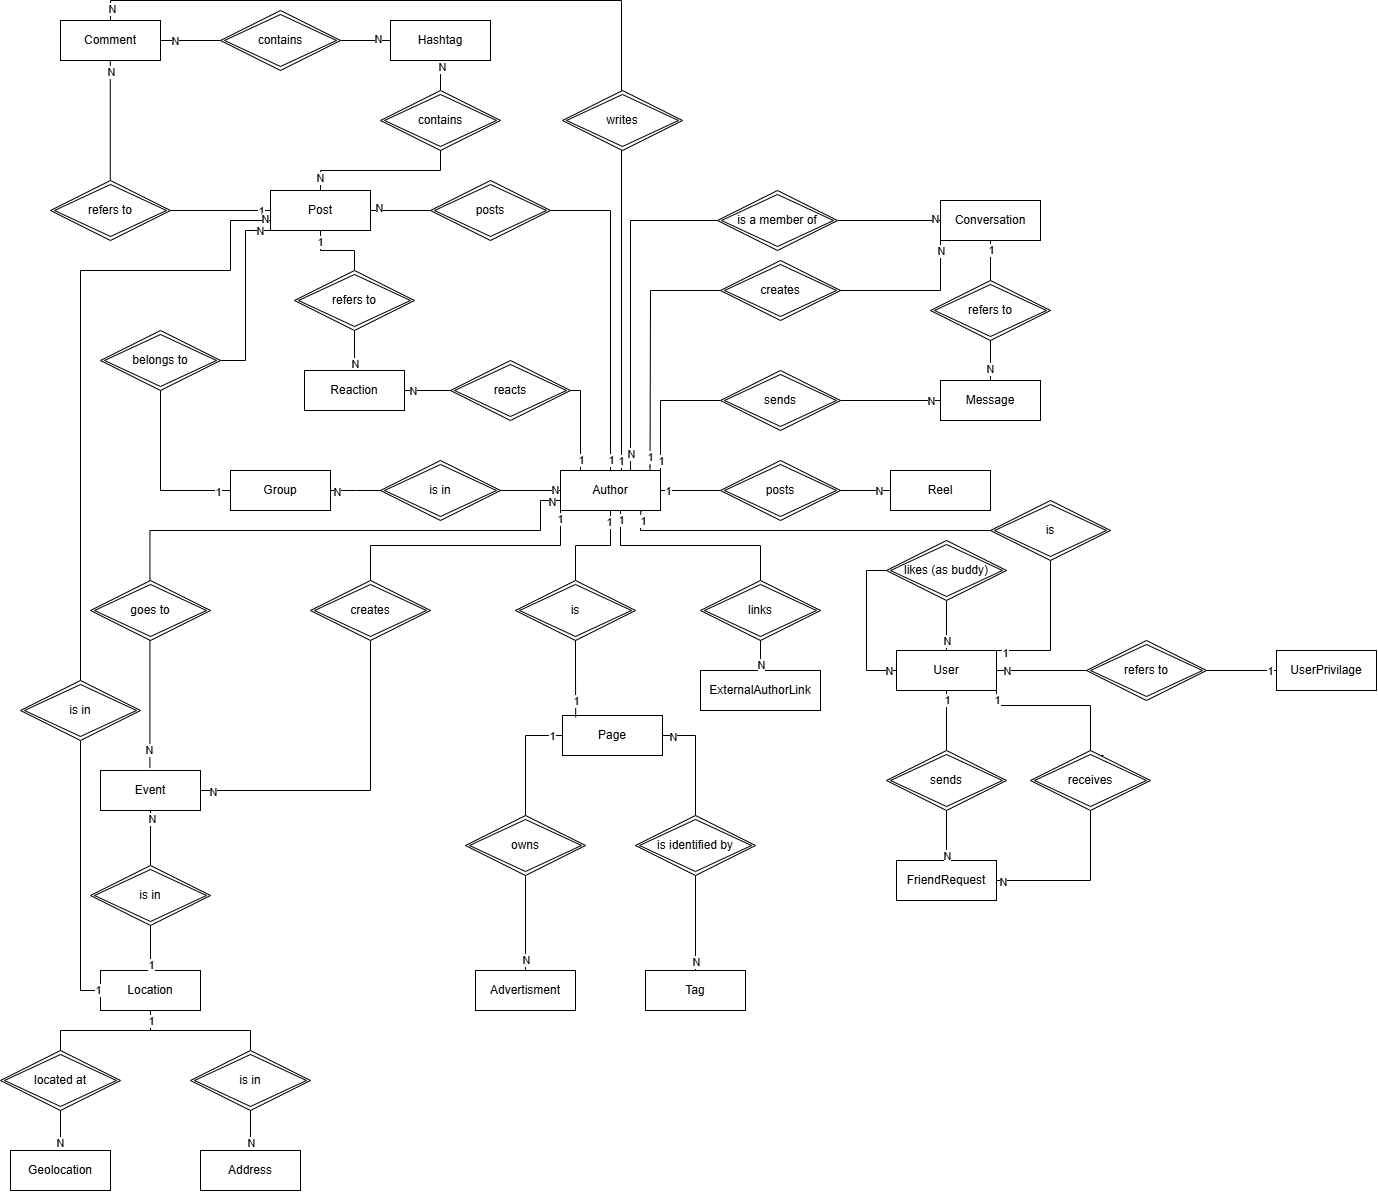
\includegraphics[width=0.95\textwidth]{images/erd_8_1.png}
    \end{center}
    \caption{Zaktualizowany ERD}
    \label{fig:new_erd}
\end{figure}


\subsection{Update schematu relacji}

Na podstawie nowego ERD'a \ref{fig:schemat_relacji} stary schemat relacji został uaktualniony, zostały usunięte błędy z poprzedniego oraz zwiększona czytelność.

\begin{figure}[htbp]
    \begin{center}
        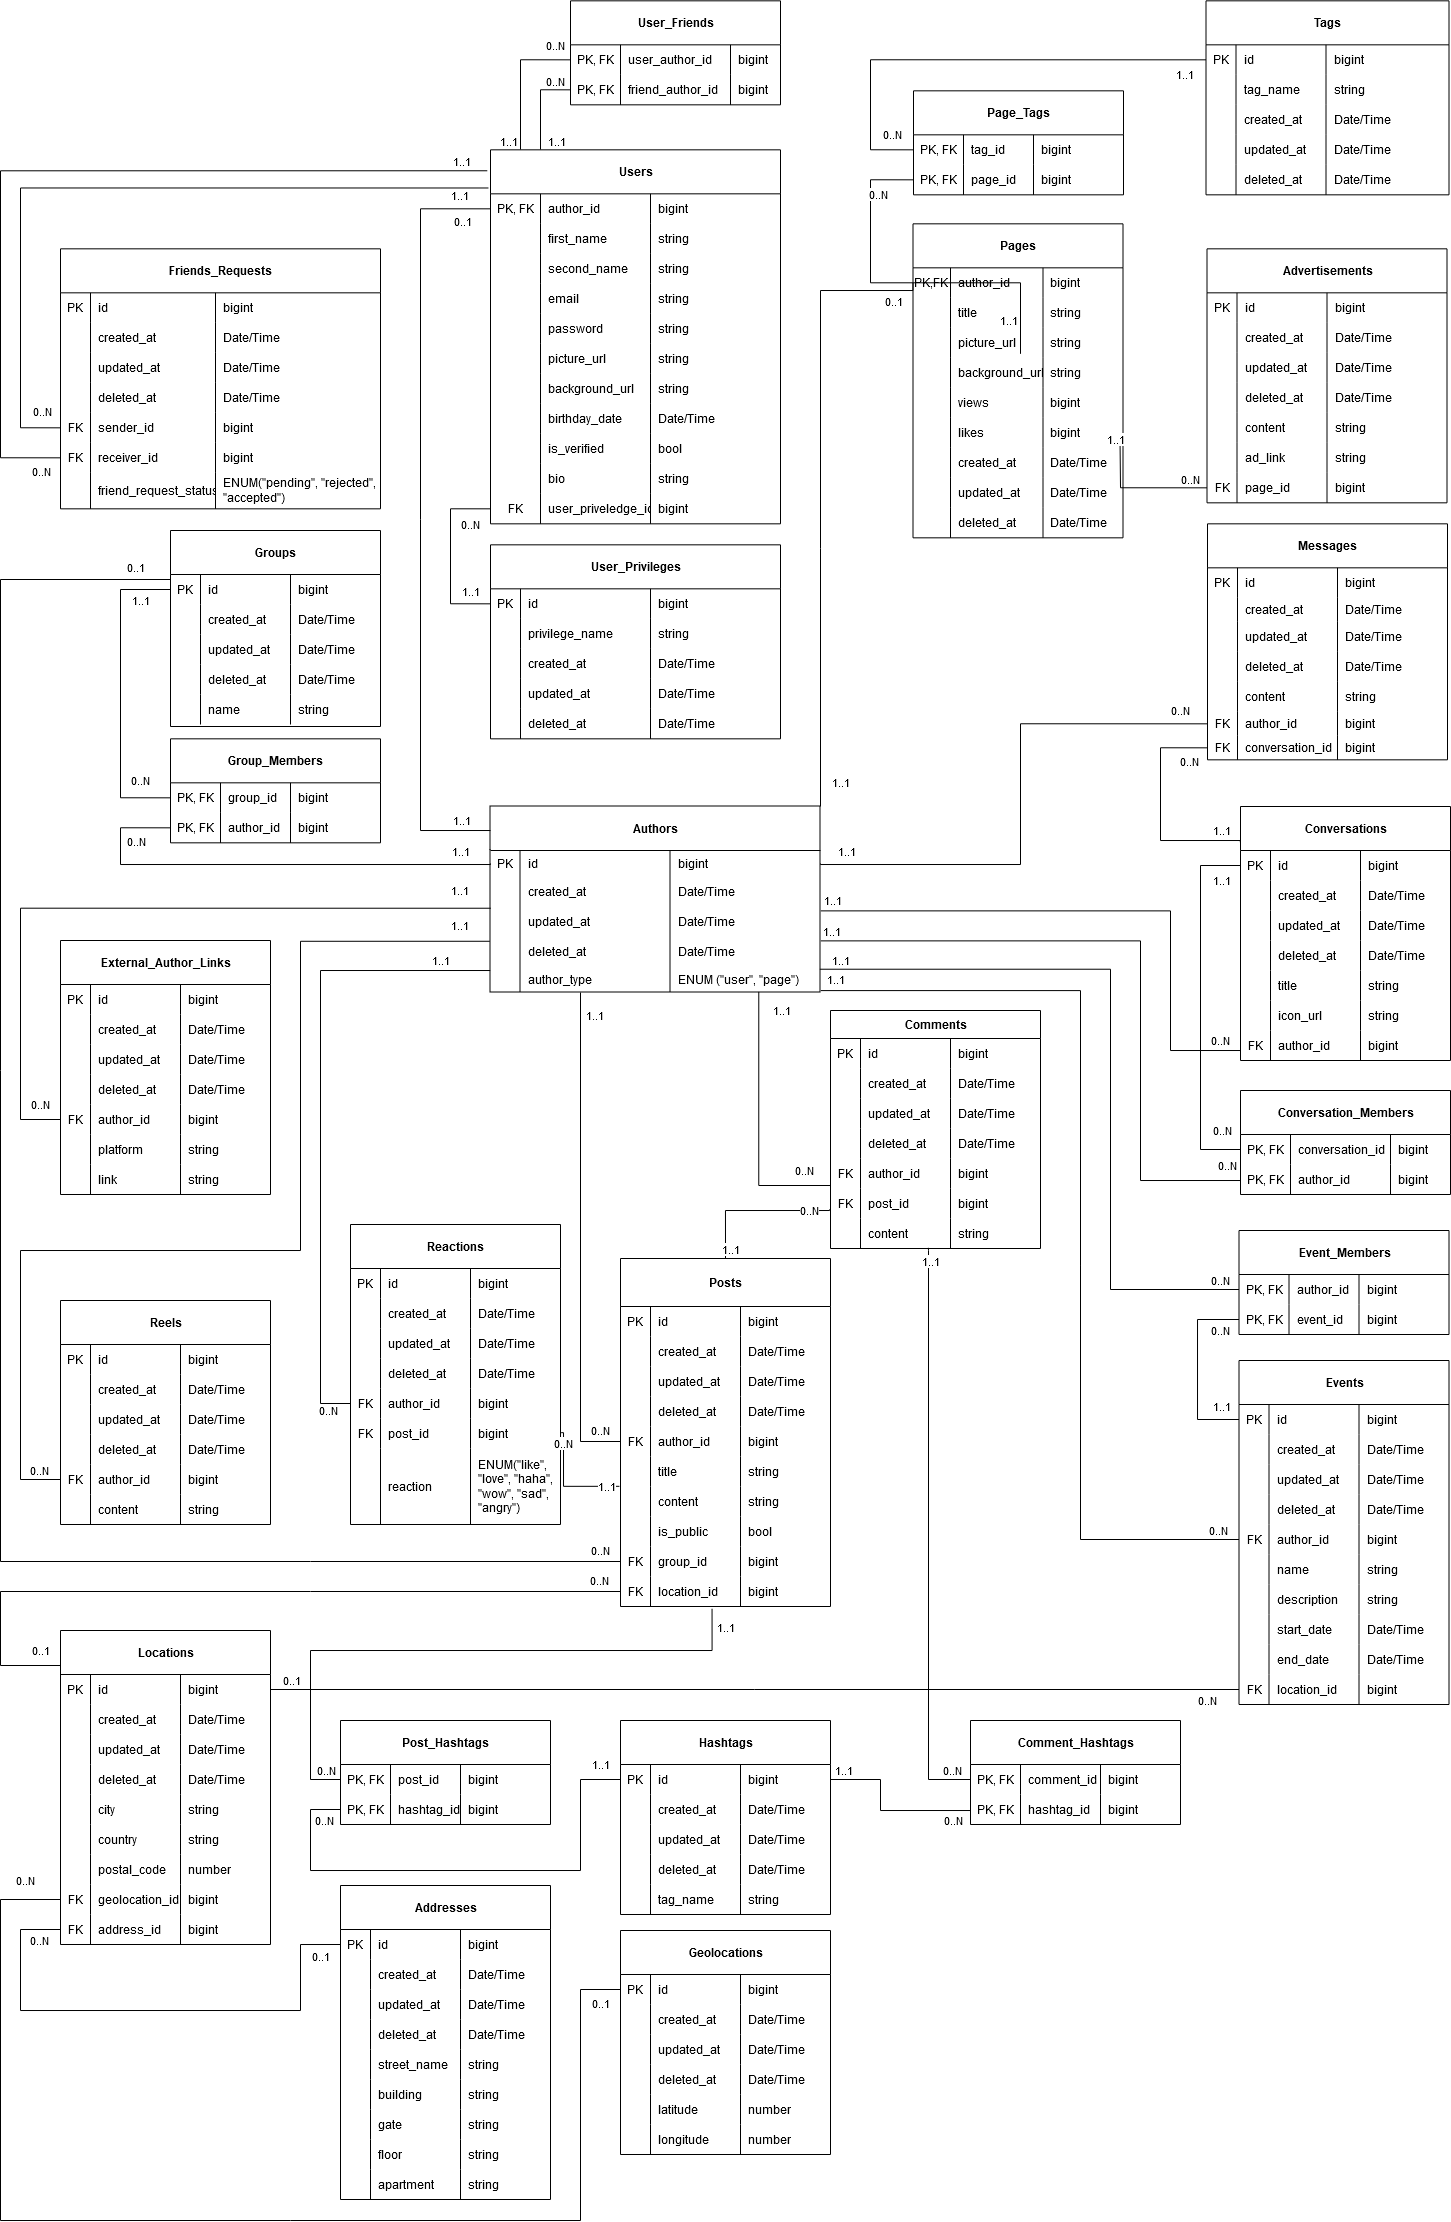
\includegraphics[width=0.95\textwidth]{images/DiagramBazyDanych_8_2.png}
    \end{center}
    \caption{Poprawiony schemat relacji bazy danych serwisu społecznościowego}
    \label{fig:schemat_relacji}
\end{figure}

\subsection{Weryfikacja i aktualizacja więzów integralności}

Aby zapewnić integralność więzłów upewniliśmy się, że:
\begin{itemize}
    \item Każda encja ma unikalny identyfikator \texttt{PK}, który jest unikalny i nie może być pusty
    \item Dla encji asocjacyjnych kluczem głównym jest para kluczy obcych, których dotyczy ta encja (np. \texttt{Group Members} identyfikowana jest prze \texttt{Group ID} i \texttt{Author ID})
    \item W przypadku relacji \texttt{1-N}  i \texttt{1-1} uwzględniamy \texttt{FK} jednej z encji w atrybutach drugiej z nich
    \item Zastosowanie \texttt{usuwania kaskadowego} sprawia, że rekordy podrzędne usuną się automatycznie, gdy usunięty zostanie rekord nadrzędny (np. gdy zostanie usunięty \texttt{Author} usunięte zostaną też jego \texttt{Posty}, a co za tym idzie też \texttt{Komentarze} i \texttt{Reakcje} dotyczące tych postów)
\end{itemize}

\newpage

\section{Etap 9: Faza logiczna II}

\subsection{Przetworzenie struktury bazy danych sprzed modyfikacji do zgodnej z nowymi wymaganiami}

Naszą bazę ulepszyliśmy w taki sposób:

\begin{itemize}
    \item dodaliśmy user\_followers - tabela asocjacyjna, która przechowuje informacje o tym, kto obserwuje kogo
    \item article, w tym section
    \item przenieśliśmy niektóre dane z tabeli Location do Address
\end{itemize}

Dodaliśmy możliwość śledzenia użytkowników, którzy obserwują danego użytkownika. Dzięki temu użytkownik może śledzić swoich ulubionych autorów.

Nasi użytkownicy mogą tworzyć długie artykuły składające się z wielu sekcji (które mają nagłówek oraz treść).

Oraz teraz geoloakalizacja jest dodatkowo wyrażana przez Point z PostGIS, pozwoli to nam na wykonanie zapytania o np. wydarzenia w promieniu \textit{n} metrów. Przenieśliśmy również część danych z Location do Address, aby ułatwić zarządzanie danymi.

Opracowaliśmy więc skrypt DDL przetwarzający strukturę starej bazy danych do nowej.

\begin{lstlisting}
    BEGIN;

DROP TABLE IF EXISTS public.user_followed CASCADE;

DROP TABLE IF EXISTS public.article_hashtags CASCADE;

DROP TABLE IF EXISTS public.articles CASCADE;

DROP TABLE IF EXISTS public.sections CASCADE;

ALTER TABLE
    IF EXISTS public.addresses DROP COLUMN IF EXISTS city;

ALTER TABLE
    IF EXISTS public.addresses DROP COLUMN IF EXISTS country;

ALTER TABLE
    IF EXISTS public.addresses DROP COLUMN IF EXISTS postal_code;

ALTER TABLE
    IF EXISTS public.geolocations DROP COLUMN IF EXISTS geom;

ALTER TABLE
    IF EXISTS public.locations
ADD
    COLUMN city character varying(100) COLLATE pg_catalog."default";

ALTER TABLE
    IF EXISTS public.locations
ADD
    COLUMN country character varying(100) COLLATE pg_catalog."default";

ALTER TABLE
    IF EXISTS public.locations
ADD
    COLUMN postal_code character varying(20) COLLATE pg_catalog."default";

DROP SEQUENCE IF EXISTS public.sections_id_seq;

DROP SEQUENCE IF EXISTS public.articles_id_seq;

END;
\end{lstlisting}

\subsection{Przykładowe zapytania}
\begin{itemize}
    \item 10 najdłuższych artykułów z ostatnich 30dni
    \item Artykuły najbardziej popularnego autora
    \item Wydarzenia w promieniu 100km
    \item Autorzy, którzy napisali najwięcej artykułów
    \item Posty z 5 najbliższych lokalizacji
    \item Użytkownik z największą liczbą obserwujących
\end{itemize}

\begin{figure}[H]
    \centering
    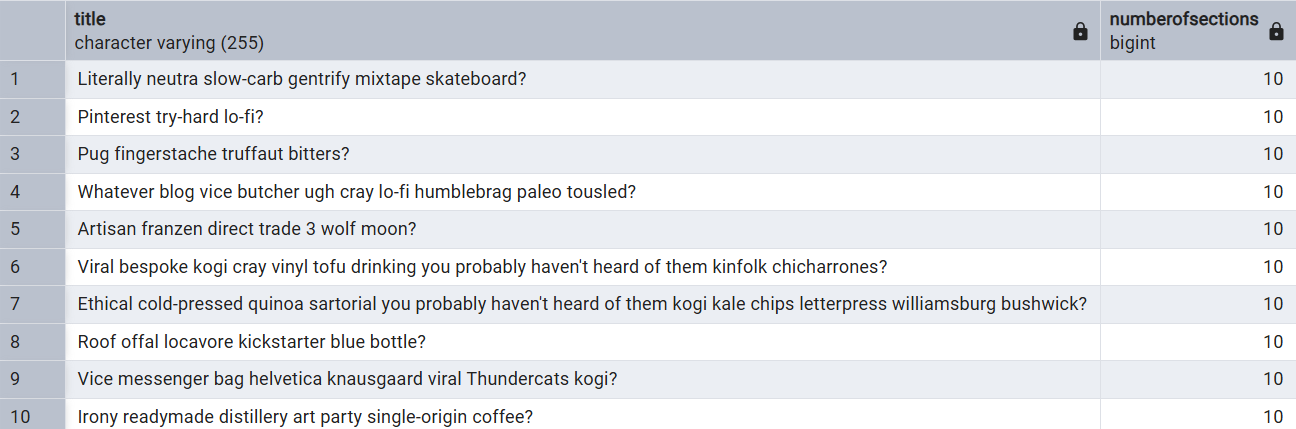
\includegraphics[width=\textwidth]{images/top_10_longest_articles_from_last_30days.png}
    \caption{Wynik kwerendy wyszukującej 10 najdłuższych artykułów z ostatnich 30dni}
    \label{fig:sql9_1}
\end{figure}

\begin{figure}[H]
    \centering
    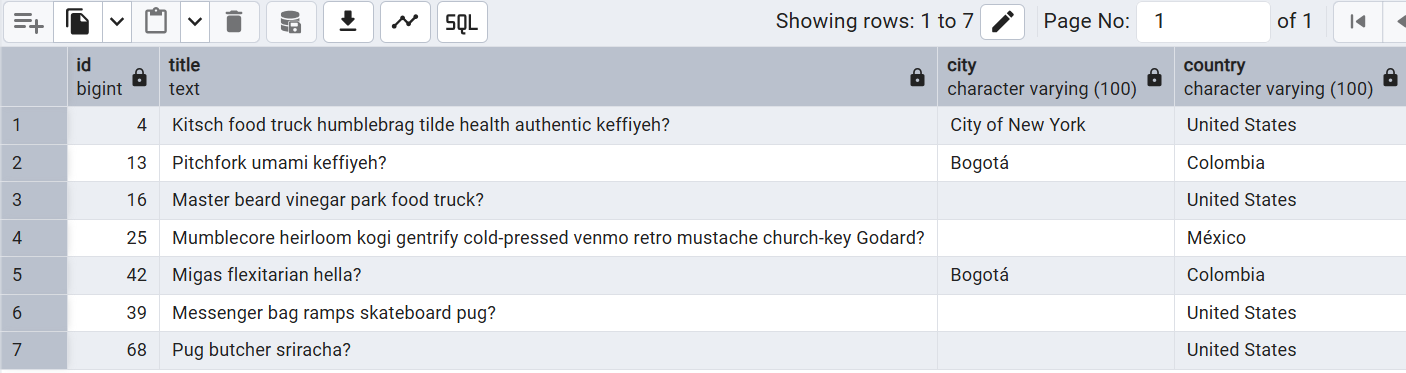
\includegraphics[width=\textwidth]{images/post_from_5_nearest_locations.png}
    \caption{Wynik kwerendy wyszukującej posty z najbliższych 5 lokalizacji}
    \label{fig:sql9_2}
\end{figure}

\begin{figure}[H]
    \centering
    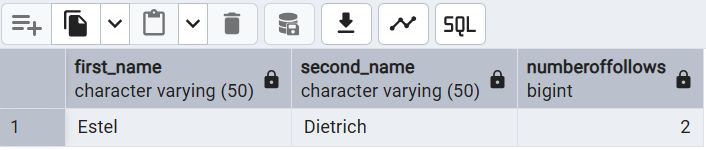
\includegraphics[width=\textwidth]{images/user_with_most_follows.png}
    \caption{Wynik kwerendy wyszukującej użytkownika z największą ilością obserwujących}
    \label{fig:sql9_3}
\end{figure}

\section{Etap 10: Nierelacyjne bazy danych - faza wstępna}

Nasz wybór padł na \textbf{MongoDB}, które według nas najlepiej sprawdzi się przy okazji tworzenia bazy dla serwisu społecznościowego. Do komunikacji z bazą wykorzystamy \textit{Pythona}.

Najbardziej optymalnym rozwiązaniem byłoby rozdzielenie danych między różne typy baz. Niektóre dane najlepiej przechowywać w bazie relacyjnej, inne w nierelacyjnej - na przykład dokumentowej lub grafowej - w zależności od ich struktury i zastosowania.

\begin{table}[htbp]
    \begin{tabular}{|l|l|}
        \hline
        \multicolumn{1}{|c|}
        {\textbf{Zalety}}                         & \multicolumn{1}{c|}{\textbf{Wady}}           \\ \hline
        Skalowanie horyzontalne                   & Brak zdefiniowanego schematu jaki jest w SQL \\ \hline
        Wysoka wydajność odczytu i zapisu         & Denormalizacja niektórych tabel              \\ \hline
        Obsługa ACID                              & Duży ruch = duże koszty                      \\ \hline
        Dobre wsparcie dla technologii np. Python &                                              \\ \hline
    \end{tabular}
    \caption{Plusy i minusy MongoDB}
    \label{table:prosAndConsOfMongoDB}

    \textbf{Założenia} (podobnie jak w przypadku relacyjnej bazy): chcemy aby baza mogła być wdrożona w jakiś serwis społecznościowy oraz aby miała dobrą wydajność, ponieważ wpyłwa to na doświadczenie użytkownika.

    \textbf{Ograniczenia}: naszym zdaniem, tak jak poprzednio, ogranicza nas to, że baza musi być w całości w NoSQL. Tymczasem - jak wcześniej wspomniano - najlepiej stworzyć bazy dedykowane dla danych tabel. Problematyczne może być tworzenie \texttt{constraints}, ponieważ bazy NoSQL nie wymagają od nas tworzenia schematów danych. W tym wypadku będziemy mieli \textbf{kolekcje} zamiast tabel i \textbf{dokumenty} zamiast wierszy. Oznacza to, że będziemy musieli zadbać sami o \textbf{integralność danych}.
\end{table}

\section{Etap 11 - Faza konceptualna i fizyczna}

\subsection{Definicja i wdrożenie struktur przechowywania danych w wybranej technologii nierelacyjnej.}

Wdrożyliśmy odpowiedniki struktur SQL w MongoDB (NoSQL). W bazie danych MongoDB nie ma tabel, a dokumenty, które są przechowywane w kolekcjach. Dokumenty są przechowywane w formacie JSON, co pozwala na przechowywanie zagnieżdżonych obiektów. Ten bardziej elastyczny sposób przechowywania danych pozwolił nam między innymi na przechowywanie User'a i Page'a w bardziej wygodny sposób.

Definiować związki można przez dodanie listy powiązanych \texttt{id} z obiektem lub przez denormalizację. Wybór jest zależny od tego, jak będą pobierane dane. Na przykład, kiedy mamy komentarz, lepiej będzie dodać autora komentarza jako mały obiekt z jego najważniejszymi danymi, takimi jak:

\begin{itemize}
    \item username lub imie, nazwisko albo email
    \item zdjęcie
\end{itemize}

Umieszczanie listy interesujących nas \texttt{id} w obiekcie przyda się, jeśli dane będą pobierane z serwera. Na przykład mamy zakładke z requestami do znajomych, wchodzimy w nią i przed renderem widoku pobieramy dane z API, wybierając kokretne obiekty z bazy. Warunkiem jest to, że user jest jakoś przechowywany.

Wykorzystane mechanizmy zapewnienia spójności:
\begin{itemize}
    \item spójność ostateczna: w międzyczasie mogą wystąpić niespójności, ale w niedalekiej przyszłości będą one spójne
    \item spójność natychmiastowa: wszystkie zmiany są od razu aplikowane na wszystkich serwerach
    \item spójność przez większość: jeśli większość serwerów powie, że dane są w porządku, to wtedy dane są spójne
\end{itemize}

Z tych mechanizmów wynika problem rozproszenia, tutaj pojawia się twierdzenie CAP, mówiące, że w systemie rozproszonym można spełnić maksymalnie 2 z 3 warunków:

\begin{itemize}
    \item C - consistent (spójność)
    \item A - available (dostępność)
    \item P - partition (tolerancja na partycjonowanie)
\end{itemize}

Nie ma jednoznaczenej odpowiedzi, które najlepiej wybrać z tych dwóch, ponieważ jest to zależne od przeznaczenia bazy.

\begin{quotation}
    "Systemy baz danych zaprojektowane z tradycyjnymi gwarancjami ACID, takimi jak RDBMS, wybierają spójność nad dostępność, natomiast systemy zaprojektowane wokół filozofii BASE, wspólne w ruchu NoSQL, na przykład, wybierają dostępność zamiast spójności \cite{wikiAboutBase}."
    \textit{CAP\_theorem, en.wikipedia.org}
\end{quotation}

ACID (Atomicity, Consistency, Isolation, Durability) to dobrze znany z tradycyjnych baz danych model, który zapewnia pełną spójność danych. W przypadku NoSQL, zamiast ACID, mówimy o BASE (Basically Available, Soft state, Eventually consistent), który skupia się bardziej na dostępności danych.

\begin{table}[h!]
    \centering
    \begin{tabular}{|l|c|c|}
        \hline
        \textbf{Cechy}           & \textbf{ACID}                   & \textbf{BASE}                   \\ \hline
        \textbf{Spójność danych} & Natychmiastowa                  & Ostateczna                      \\ \hline
        \textbf{Dostępność}      & Ograniczona w razie problemów   & Zawsze dostępne                 \\ \hline
        \textbf{Wydajność}       & Mniejsza, szczególnie w skali   & Wyższa, dzięki kompromisom      \\ \hline
        \textbf{Zastosowanie}    & Bankowość, finanse, systemy ERP & Media społecznościowe, big data \\ \hline
    \end{tabular}
    \caption{Porównanie paradygmatów ACID i BASE}
    \label{tab:acid_base_comparison}
\end{table}

Model Base zdecydowanie bardziej pasuje do dynamicznej struktury serwisów społecznościowych, gdzie dostępność danych jest kluczowa, a spójność danych nie jest tak ważna.

\subsection{Prezentacja przykładowych zapytań}

Poniżej podaliśmy odpowiedniki komend SQL w MongoDB (NoSQL).

\begin{itemize}
    \item SELECT * FROM users $\rightarrow$ db.users.find()
    \item SELECT * FROM users WHERE age $<$ 18 $\rightarrow$ db.users.find({ age: { \$lt: 18 } })
    \item INSERT INTO users (krotka) VALUES (dane) $\rightarrow$ db.users.insertOne({ dane: "w json" })
    \item CREATE INDEX idx\_deleted\_at ON users (deleted\_at) $\rightarrow$ db.users.createIndex({ deleted\_at: 1 })
\end{itemize}

\section{Etap 12: Faza fizyczna }

\quad Standardowo kod można zobaczyć w repozytorium na gicie: \href{https://github.com/lukaszfabia/social_media_db}{social media db}. Skrypt łączący się z bazą danych przechowywaną w chmurze i generujący rekordy do kolekcji to main.py. Wykorzystuje on funkcje napisane w seeder.py.\\

\quad Mając wcześniej napisaną strukturę modeli przy użyciu pydantic należało napisać funkcje generujące dane do bazy. Można je było podzielić na dwa rodzaje:

\begin{enumerate}
    \item Funkcje generujące rekordy do kolekcji.
    \item Funkcje generujące rekordy dla wszystkich rekordów w danej kolekcji, przykładowo dodawanie konwersacji dla każdego użytkownika.
\end{enumerate}

Zapełnianie bazy danych dużą ilością danych zajmuje stosunkowo dużo czasu, może to być spowodowane przez wywołania które tworzą listy użytkowników dla np. eventów, innym podejrzeniem może być nieoptymalnie napisany kod. \\


\textbf{Język}: \href{https://www.python.org/}{Python}

\textbf{Generowanie sztucznych danych}: \href{https://faker.readthedocs.io/en/master/}{Faker}


\bibliography{sample}
\bibliographystyle{abbrv}

\end{document}



